% concatenated from V2-LeakyForcingHopiRectangles.tex
\documentclass[11pt]{article}
\bibliographystyle{plain}


\usepackage{cite}

\usepackage{graphicx} % Required for inserting images
\usepackage{amssymb,latexsym,amsfonts,amsmath,amsthm}
\usepackage{amssymb,latexsym,amsfonts}
% \usepackage{fullpage}

            

\usepackage{hyperref}
\usepackage[dvipsnames]{xcolor}
\usepackage{tikz}
\usetikzlibrary{graphs}
\usetikzlibrary{graphs.standard}
\usetikzlibrary{shapes.multipart,shapes.geometric,topaths,calc, positioning, decorations.pathreplacing, calligraphy}
\usepackage{ragged2e}
\usepackage{blindtext}
\usepackage{soul}
\usepackage{array}
\usepackage{tikz,lipsum,lmodern}
\usetikzlibrary{graphs}
\usetikzlibrary{matrix}
\usetikzlibrary{graphs.standard}
\usepackage{hyperref}
\usepackage{mathalpha}
\usepackage{array}
\usepackage{float}
%\usepackage[cal=bickham,calscaled=.96]{mathalpha}
\usepackage[most]{tcolorbox}
\usepackage[paperwidth=8.5in,paperheight=10.5 in]{geometry}
     \geometry{margin=1.in}
\usepackage{caption}
\usepackage{subcaption}
\usepackage{multicol}


\usepackage{graphicx} % Required for inserting images


\newcommand\Zf[1]{Z(#1)}
\newcommand\Zl[1]{Z_{(\ell)}(#1)}
\newcommand\Zone[1]{Z_{(1)}(#1)}
\newcommand\Ztwo[1]{Z_{(2)}(#1)}
\newcommand\Znum[2]{Z_{(#2)}(#1)}



% \usepackage{amscd,mathtools,cases}
% \usepackage{amssymb,latexsym,amsfonts,amsmath,amsthm}
% \bibliographystyle{plain}
% \usepackage{tikz}
% \usepackage{appendix}
% \usepackage{subcaption}
% \usepackage{cite}
% \usepackage{blindtext}

% \title{Leaky Zero Forcing on Induced Subgraphs of $d$-dimensional Grid Graphs}
\title{Leaky Zero Forcing on Induced Subgraphs of $d$-dimensional Grid Graphs with an Application to Hopi Rectangles}
\author{
Ryan Moruzzi, Jr.\thanks{Department of Mathematics, California State University, Northridge, USA, \\ Corresponding author. Email: \texttt{ryan.moruzzi@csun.edu}} \and Sagar Shah \thanks{California State University East Bay, Hayward, USA} \and Aaditeya Tripathi \thanks{California State University East Bay, Hayward, USA} 
}

% \author{Beth Bjorkman\thanks{Air Force Research Laboratory Sensors Directorate, Wright-Patterson Air Force Base, OH, USA (beth.morrison@us.af.mil)} \and Lei Cao\thanks{Department of Mathematics, Halmos College, Nova Southeastern University, Fort Lauderdale, FL, USA (lcao@nova.edu)} \and Franklin Kenter\thanks{Mathematics Department, United States Naval Academy, Annapolis, MD, USA (kenter@usna.edu)} \and  Ryan Moruzzi Jr\thanks{Department of Mathematics, California State University, Northridge, Northridge, CA, USA (ryan.moruzzi@csun.edu)} \and Carolyn Reinhart\thanks{Department of Mathematics and Statistics, Swarthmore College, Swarthmore, PA, USA (creinha1@swarthmore.edu)} \and Violeta Vasilevska\thanks{Department of Mathematics, Utah Valley University, Orem, UT, USA (violeta.vasilevska@uvu.edu)}
% }




\date{February 2026}
%\theoremstyle{definition} 

\theoremstyle{plain} \newtheorem{question}{Question}
\newtheorem{thm}{Theorem}
\newtheorem{cor}[thm]{Corollary}

\theoremstyle{definition}
\newtheorem{defn}[thm]{Definition}
\newtheorem{rem}[thm]{Remark}
\newtheorem{prop}[thm]{Proposition}
\newtheorem{lem}[thm]{Lemma}

\newtheorem{obs}[thm]{Observation}

\newtheorem{claim}[thm]{Claim}

% \newtheorem*{rem*}[theorem]{Remark}

\begin{document}

\maketitle

\begin{abstract}
We study zero forcing and $\ell$-leaky zero forcing on induced subgraphs of $d$-dimensional grid graphs. Using $\ell$-leaky forts, we prove structural results showing that for $\ell \le 2d-1$, every nonempty $\ell$-leaky fort in an induced subgraph of $P_{n_1}\square\cdots\square P_{n_d}$ intersects the boundary of the graph. These results give general bounds and, in certain settings, exact values for the $\ell$-leaky forcing number of induced subgraphs. Motivated by this framework, we introduce an integer lattice based definition of the Hopi rectangle graphs $HD(a,b)$ as induced subgraphs of $P_{a+b}\square P_{a+b}$. For this particular family of graphs, we show that the zero forcing number equals the maximum nullity, and we completely characterize the $\ell$-leaky forcing number for all $\ell\ge 1$.

\end{abstract}

\noindent\textbf{Keywords:} Zero forcing, maximum nullity, leaky forcing, forts, $d$-dimensional grid graphs, Aztec rectangle graphs, Hopi rectangle graphs.

\noindent{\bf AMS subject classification:} 05C50, 05C76.


\section{Introduction}
Zero forcing on a graph is an iterative graph coloring process where one begins with a subset of vertices colored blue and repeatedly applies a color change rule with the goal of eventually coloring the entire graph blue. The standard color change rule is as follows: if a blue vertex has exactly one non–blue neighbor, then that neighbor is \emph{forced} to become blue. This forcing may occur over multiple rounds until no further forces are possible. If an initial blue set of vertices is able to color all other vertices of $G$, it is called a \emph{zero forcing set}, with the minimum cardinality of such a set being called the \emph{zero forcing number} of $G$, denoted $Z(G)$.

Although zero forcing can be studied purely from a graph-theoretic perspective, it is closely connected to linear algebra through its relationship with the maximum nullity of a graph. This connection was first established by the AIM (American Institute of Mathematics) Minimum Rank–Special Graphs Work Group \cite{AIMMINIMUMRANKWorkgroup}, who introduced zero forcing in the context of the minimum rank and maximum nullity. They showed that the zero forcing number provides a graph-theoretic upper bound on the maximum nullity, and since then, the topic of zero forcing has flourished into a rich area of research in its own right. 

Zero forcing can also be viewed as a model for the spread of information in a network, and results in this area have found applications in contexts such as quantum control \cite{QuantumControl} and search algorithms \cite{SearchTrees}. In such applications, one may be concerned with the presence of faulty vertices that obstruct propagation. Therefore, the notion of a ``leaked'' or ``faulty'' vertex was introduced in \cite{KenterOGpaper}, leading to a variation of zero forcing known as \emph{leaky zero forcing} (or simply \emph{leaky forcing}) which follows the same color change rule as zero forcing, except that leaked vertices are not allowed to perform forces. The main question in this setting is: what is the minimum number of vertices required to force the graph despite the presence of $\ell$ leaked vertices, regardless of where those leaks occur? The minimum number needed is called the \emph{$\ell$-leaky forcing number} of a graph $G$, and is denoted $Z_{(\ell)}(G)$. As in standard zero forcing, \textit{forts} are key objects of interest. A \emph{fort} is a subset of vertices whose complement cannot force into it under the standard color change rule. In the leaky setting, understanding the structure of the analogous leaky forts is an essential tool for determining $Z_{(\ell)}(G)$. This concept of leaky forcing has attracted much recent attention; see, for instance, \cite{KenterOGpaper,Reslience,GeneralLeaky,herrman2024leakyforcingresiliencecartesian,QdLeaky}, as well as related variations in \cite{elias2024leakypositivesemidefiniteforcing}.

In this work, we study the zero forcing and leaky forcing number of induced subgraphs of $d$-dimensional grid graphs in general, then focus our study on a particular family of induced subgraphs of the $2$-dimensional grid $P_{n_1}\square P_{n_2}$. Our interest in this setting was motivated by the family of planar graphs known as Aztec rectangle graphs, which can be viewed as induced subgraphs of $2$-dimensional grid graphs. These graphs arise as a natural generalization of the Aztec diamond graph, originally studied from a combinatorial perspective through the enumeration of domino tilings of the Aztec diamond, the dual of the Aztec diamond graph \cite{FirstMentionAD,AztecDiamondGraphs-Benkart}. More recently, extensions to tilings of double Aztec rectangles have also been studied \cite{DoubleAztecRect}.

The paper is organized as follows. In Section \ref{sec:background}, we provide definitions and known results that are used in our work. In Section \ref{sec:FortsInducedSubgraphs}, we establish structural results describing leaky forts in induced subgraphs of $d$-dimensional grid graphs, which we then use to characterize the leaky forcing number of such induced subgraphs. In Section \ref{sec:ApplicationHopiRec}, we further motivate our focus on Aztec rectangle graphs, establish this family as an induced subgraph of $2$-dimensional grid graphs, and obtain an upper bound on the minimum rank. In Section \ref{sec:ZFonHopiRectanlges}, we apply our general results to prove equality of the zero forcing number and maximum nullity, and we fully characterize the leaky forcing numbers for Aztec rectangle graphs. We conclude in Section \ref{sec:FutureWork} with directions for future work.



\section{Preliminaries}\label{sec:background}

All graphs we consider are finite, simple, and undirected. For a graph $G$, we write $V(G)$ and $E(G)$ for its \emph{vertex} and \emph{edge sets}, respectively, and $|V(G)|$ for the \emph{size} of $G$. For $v\in V(G)$, let $N_G(v)$ denote the \emph{open neighborhood} of $v$ in $G$ which are vertices incident to $v$, and $\deg_G(v)=|N_G(v)|$ its degree. If $A\subseteq V(G)$, then $G[A]$ denotes the \emph{induced subgraph} of $A$ in $G$ which is a graph such that for any pair of vertices in $A$, if those vertices are adjacent in $G$, then they must be adjacent in $A$. An \emph{edge covering} by subgraphs of $G$ is a collection of subgraphs $H_1,\dots,H_t$ with $E(G)=\bigcup_{i=1}^t E(H_i)$. We write $P_n$ for the path on $n$ vertices and $C_n$ for the cycle on $n$ vertices. The \emph{$d$-dimensional grid graph} is the Cartesian product
$P_{n_1}\square P_{n_2}\square \cdots \square P_{n_d}$. Its vertex set is
$V(P_{n_1})\times \cdots \times V(P_{n_d})$, and $(x_1,\ldots,x_d)\sim (y_1,\ldots,y_d)$ if and only if
$(x_1,\ldots,x_d)$ and $(y_1,\ldots,y_d)$ differ in exactly one coordinate, say the $k$th, and
$x_k\sim y_k$ in $P_{n_k}$.


Let $\mathcal{S}(G)$ be the set of real symmetric matrices whose graph is $G$, that is 
$$S(G) = \{A= (a_{i,j})\in \mathbb{R}^{n\times n} : A = A^T,\ a_{i,j}\ne 0 \text{ iff } ij\in E(G)\ \text{and} \ i\ne j\},$$

\noindent and the \emph{minimum rank} and \emph{maximum nullity} of $G$ given as
\[
mr(G)=\min\{\text{rank}(A) : A\in \mathcal{S}(G)\},\qquad
M(G)=\max\{\text{null}(A) : A\in \mathcal{S}(G)\}  .
\]

Recall that zero forcing is an iterative coloring process on $G$ where, starting with an initial blue set $B\subseteq V(G)$, if a blue vertex $u$ has exactly one white neighbor $v$, then $u$ \emph{forces} $v$ (written $u\to v$), turning $v$ blue. A \emph{chronological set of forces} is an ordering of all such forces that can be applied round by round. $B$ is a \emph{zero forcing set} if the vertices in $B$ can force the entire graph blue, and the minimum size of a such zero forcing set is the \emph{zero forcing number of G}, denoted $Z(G)$. 


In 2008, an AIM Special Graphs Work group determined the following connection between the maximum nullity $M(G)$ and the zero forcing number $Z(G)$ of a graph, which subsequently ushered in the study of zero forcing in its own right in the context of maximum nullity and minimum rank.   

\begin{prop}[Proposition 2.4, \cite{AIMMINIMUMRANKWorkgroup}]\label{thm:NullityInequality}
    For any graph $G$, $M(G)\le Z(G)$.
\end{prop}


In 2019, the notion of a leaky vertex to hinder the zero forcing process in graphs, akin to faulty sensors while observing a network, was introduced \cite{KenterOGpaper}. Leaky zero forcing follows the same color change rule as zero forcing, with the added notion of allowing up to $\ell$ vertices to be designated as leaks, meaning they are vertices that are unable to perform a force. The minimum size of an initial blue set that is able to force the entire graph blue for every placement of $\ell$ leaks is called the \emph{$\ell$-leaky forcing number}, denoted $Z_{(\ell)}(G)$. We collect here several results about leaky forcing that will be useful throughout this paper. First, Lemma~\ref{lem:moreleaksinq} gives us that leaky forcing numbers are monotonic in terms of the number of leaks. Lemma~\ref{lem:lowdegree} gives that vertices of particular degree must always belong to particular leaky forcing sets. Finally, Theorem~\ref{prop:twoways} gives a way to show that an initial set is a $1$-leaky set by way of unique ways to force each vertex. 

\begin{lem}[Lemma 2.1, \cite{KenterOGpaper}]
\label{lem:moreleaksinq}
For any graph $G$ on $n$ vertices,
\[  
Z_{(0)}(G) \leq Z_{(1)}(G) \leq Z_{(2)}(G) \leq \cdots \leq Z_{(n)}(G).  
\]
\end{lem}


\begin{lem}[Lemma 2.4, \cite{KenterOGpaper}] \label{lem:lowdegree}
Let $G$ be a graph and choose $\ell \geq 0$. Then every $\ell$-leaky forcing set contains all vertices of degree at most $\ell$.
\end{lem}



\begin{thm}[Theorem 2.3, \cite{Reslience}]\label{prop:twoways}
A set $B$ is a $1$-leaky forcing set if and only if for every $v \in V(G)\setminus B$, there exist distinct forces $x \to v$ and $y \to v$ with $x \neq y$ in the set of all forces originating from $B$.
\end{thm}





In our work on induced subgraphs of the $d$-dimensional grid, to fully characterize the $\ell$ leaky forcing number, particularly when $\ell\ge 2$, we utilize the notion of \emph{leaky forts}. Intuitively, a leaky fort is a vertex set $S$ that is resistant to forcing from the outside. Specifically, if all vertices in $V(G)\setminus S$ are blue, then no force can occur into $S$. The formal definition for a leaky fort is the following. 

\begin{defn}\label{def:lfort}
An \emph{$\ell$-leaky fort} in a graph $G$ is a subset $S\subseteq V(G)$ such that
\[
\left|\left\{x\in V(G)\setminus S:\ \left|N_G(x)\cap S\right|=1\right\}\right|\le \ell.
\]
\end{defn}

An illustration of a fort and an example of a 3-leaky fort of an induced subgraph of the $2$-dimensional grid $P_{5} \square P_{5}$ can be seen in Figure \ref{fig:LeakyForts}. The next result establishes the connection between leaky forts and the $\ell$-leaky forcing number of a graph, which will play a crucial role in determining $\ell$-leaky forcing numbers in Section~\ref{sec:FortsInducedSubgraphs}.

\begin{prop}[Proposition 2.3, \cite{KenterOGpaper}]\label{prop:LeakyForcingSetIntersectsForts}
For any graph $G$, a subset of vertices $S$ of $G$ is an $\ell$-leaky forcing set if and only if $S$ intersects every $\ell$-leaky fort of $G$.
\end{prop}

\begin{figure}[h!]
    \centering

\tikzset{every picture/.style={line width=0.75pt}} %set default line width to 0.75pt        

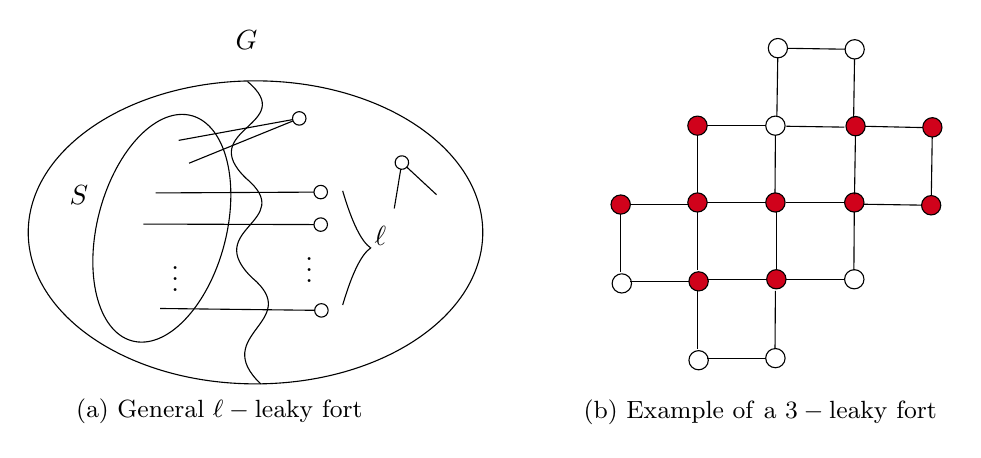
\begin{tikzpicture}[x=0.75pt,y=0.75pt,yscale=-1,xscale=1]
%uncomment if require: \path (0,3166); %set diagram left start at 0, and has height of 3166

%Straight Lines [id:da03672671764989199] 
\draw    (191.5,1930) -- (244.58,1908.42) ;
%Straight Lines [id:da8050226245565235] 
\draw    (186.5,1919) -- (244.58,1908.42) ;
%Shape: Ellipse [id:dp7025065750291334] 
\draw   (114,1963.33) .. controls (114,1923.02) and (163.02,1890.33) .. (223.5,1890.33) .. controls (283.98,1890.33) and (333,1923.02) .. (333,1963.33) .. controls (333,2003.65) and (283.98,2036.33) .. (223.5,2036.33) .. controls (163.02,2036.33) and (114,2003.65) .. (114,1963.33) -- cycle ;
%Curve Lines [id:da807344510283815] 
\draw    (222,1985.33) .. controls (247,2006.33) and (201,2012.33) .. (226,2036.33) ;
%Curve Lines [id:da43608542481098445] 
\draw    (219,1937.33) .. controls (244,1958.33) and (197,1961.33) .. (222,1985.33) ;
%Curve Lines [id:da959365123946525] 
\draw    (219.67,1890.67) .. controls (244.67,1911.67) and (194,1913.33) .. (219,1937.33) ;
%Shape: Ellipse [id:dp6567127404232125] 
\draw   (147.79,1955.63) .. controls (154.98,1925.5) and (174.5,1903.63) .. (191.39,1906.79) .. controls (208.28,1909.95) and (216.15,1936.94) .. (208.96,1967.08) .. controls (201.77,1997.21) and (182.25,2019.07) .. (165.35,2015.91) .. controls (148.46,2012.75) and (140.6,1985.76) .. (147.79,1955.63) -- cycle ;
%Shape: Circle [id:dp790725579330702] 
\draw  [fill={rgb, 255:red, 255; green, 255; blue, 255 }  ,fill opacity=1 ] (241.33,1908.42) .. controls (241.33,1906.62) and (242.79,1905.17) .. (244.58,1905.17) .. controls (246.38,1905.17) and (247.83,1906.62) .. (247.83,1908.42) .. controls (247.83,1910.21) and (246.38,1911.67) .. (244.58,1911.67) .. controls (242.79,1911.67) and (241.33,1910.21) .. (241.33,1908.42) -- cycle ;
%Straight Lines [id:da38069210789191854] 
\draw    (310.72,1945.18) -- (294.02,1929.69) ;
%Straight Lines [id:da672090615026622] 
\draw    (290.35,1951.8) -- (294.02,1929.69) ;
%Shape: Circle [id:dp5342917443235455] 
\draw  [fill={rgb, 255:red, 255; green, 255; blue, 255 }  ,fill opacity=1 ] (293.68,1932.92) .. controls (291.9,1932.74) and (290.6,1931.14) .. (290.79,1929.35) .. controls (290.98,1927.57) and (292.58,1926.27) .. (294.36,1926.46) .. controls (296.15,1926.64) and (297.44,1928.24) .. (297.25,1930.03) .. controls (297.07,1931.81) and (295.47,1933.11) .. (293.68,1932.92) -- cycle ;
%Straight Lines [id:da022957922997620783] 
\draw    (175.33,1944.33) -- (254.92,1943.92) ;
%Shape: Circle [id:dp49472797969903337] 
\draw  [fill={rgb, 255:red, 255; green, 255; blue, 255 }  ,fill opacity=1 ] (251.67,1943.92) .. controls (251.67,1942.12) and (253.12,1940.67) .. (254.92,1940.67) .. controls (256.71,1940.67) and (258.17,1942.12) .. (258.17,1943.92) .. controls (258.17,1945.71) and (256.71,1947.17) .. (254.92,1947.17) .. controls (253.12,1947.17) and (251.67,1945.71) .. (251.67,1943.92) -- cycle ;
%Straight Lines [id:da4584372466201041] 
\draw    (169.5,1959.33) -- (254.92,1959.58) ;
%Shape: Circle [id:dp9707184803714094] 
\draw  [fill={rgb, 255:red, 255; green, 255; blue, 255 }  ,fill opacity=1 ] (251.67,1959.58) .. controls (251.67,1957.79) and (253.12,1956.33) .. (254.92,1956.33) .. controls (256.71,1956.33) and (258.17,1957.79) .. (258.17,1959.58) .. controls (258.17,1961.38) and (256.71,1962.83) .. (254.92,1962.83) .. controls (253.12,1962.83) and (251.67,1961.38) .. (251.67,1959.58) -- cycle ;
%Straight Lines [id:da22885951151879702] 
\draw    (177.5,2000) -- (255.25,2000.92) ;
%Shape: Circle [id:dp25405234279541] 
\draw  [fill={rgb, 255:red, 255; green, 255; blue, 255 }  ,fill opacity=1 ] (252,2000.92) .. controls (252,1999.12) and (253.46,1997.67) .. (255.25,1997.67) .. controls (257.04,1997.67) and (258.5,1999.12) .. (258.5,2000.92) .. controls (258.5,2002.71) and (257.04,2004.17) .. (255.25,2004.17) .. controls (253.46,2004.17) and (252,2002.71) .. (252,2000.92) -- cycle ;
\draw   (265.5,1943.33) .. controls (270,1958.61) and (274.5,1967.78) .. (279,1970.83) .. controls (274.5,1973.89) and (270,1983.06) .. (265.5,1998.33) ;
%Shape: Ellipse [id:dp06408843986926971] 
\draw  [fill={rgb, 255:red, 208; green, 2; blue, 27 }  ,fill opacity=1 ] (431.77,1911.93) .. controls (431.77,1909.37) and (433.86,1907.3) .. (436.44,1907.3) .. controls (439.02,1907.3) and (441.11,1909.37) .. (441.11,1911.93) .. controls (441.11,1914.48) and (439.02,1916.55) .. (436.44,1916.55) .. controls (433.86,1916.55) and (431.77,1914.48) .. (431.77,1911.93) -- cycle ;
%Shape: Ellipse [id:dp7199389784019377] 
\draw   (469.32,1911.93) .. controls (469.32,1909.37) and (471.41,1907.3) .. (473.99,1907.3) .. controls (476.57,1907.3) and (478.66,1909.37) .. (478.66,1911.93) .. controls (478.66,1914.48) and (476.57,1916.55) .. (473.99,1916.55) .. controls (471.41,1916.55) and (469.32,1914.48) .. (469.32,1911.93) -- cycle ;
%Straight Lines [id:da9504825391335379] 
\draw    (441.11,1911.93) -- (469.32,1911.93) ;
%Straight Lines [id:da10630953381148334] 
\draw    (436.44,1916.55) -- (436.44,1944.59) ;
%Straight Lines [id:da7337796348196598] 
\draw    (473.99,1916.55) -- (473.8,1944.59) ;
%Shape: Ellipse [id:dp6279651307054729] 
\draw  [fill={rgb, 255:red, 208; green, 2; blue, 27 }  ,fill opacity=1 ] (431.77,1948.93) .. controls (431.77,1946.37) and (433.86,1944.3) .. (436.44,1944.3) .. controls (439.02,1944.3) and (441.11,1946.37) .. (441.11,1948.93) .. controls (441.11,1951.48) and (439.02,1953.55) .. (436.44,1953.55) .. controls (433.86,1953.55) and (431.77,1951.48) .. (431.77,1948.93) -- cycle ;
%Shape: Ellipse [id:dp4267699150759492] 
\draw  [fill={rgb, 255:red, 208; green, 2; blue, 27 }  ,fill opacity=1 ] (469.32,1948.93) .. controls (469.32,1946.37) and (471.41,1944.3) .. (473.99,1944.3) .. controls (476.57,1944.3) and (478.66,1946.37) .. (478.66,1948.93) .. controls (478.66,1951.48) and (476.57,1953.55) .. (473.99,1953.55) .. controls (471.41,1953.55) and (469.32,1951.48) .. (469.32,1948.93) -- cycle ;
%Straight Lines [id:da1318818619044183] 
\draw    (441.11,1948.93) -- (469.32,1948.93) ;
%Shape: Ellipse [id:dp33128612244237954] 
\draw  [fill={rgb, 255:red, 208; green, 2; blue, 27 }  ,fill opacity=1 ] (507.32,1948.93) .. controls (507.32,1946.37) and (509.41,1944.3) .. (511.99,1944.3) .. controls (514.57,1944.3) and (516.66,1946.37) .. (516.66,1948.93) .. controls (516.66,1951.48) and (514.57,1953.55) .. (511.99,1953.55) .. controls (509.41,1953.55) and (507.32,1951.48) .. (507.32,1948.93) -- cycle ;
%Straight Lines [id:da22471099020408591] 
\draw    (479.11,1948.93) -- (507.32,1948.93) ;
%Straight Lines [id:da9824690266934843] 
\draw    (474.44,1953.55) -- (474.44,1981.59) ;
%Straight Lines [id:da31337034898968263] 
\draw    (511.99,1953.55) -- (511.8,1981.59) ;
%Shape: Ellipse [id:dp7956669259457142] 
\draw  [fill={rgb, 255:red, 208; green, 2; blue, 27 }  ,fill opacity=1 ] (469.77,1985.93) .. controls (469.77,1983.37) and (471.86,1981.3) .. (474.44,1981.3) .. controls (477.02,1981.3) and (479.11,1983.37) .. (479.11,1985.93) .. controls (479.11,1988.48) and (477.02,1990.55) .. (474.44,1990.55) .. controls (471.86,1990.55) and (469.77,1988.48) .. (469.77,1985.93) -- cycle ;
%Shape: Ellipse [id:dp1514363314856314] 
\draw   (507.32,1985.93) .. controls (507.32,1983.37) and (509.41,1981.3) .. (511.99,1981.3) .. controls (514.57,1981.3) and (516.66,1983.37) .. (516.66,1985.93) .. controls (516.66,1988.48) and (514.57,1990.55) .. (511.99,1990.55) .. controls (509.41,1990.55) and (507.32,1988.48) .. (507.32,1985.93) -- cycle ;
%Straight Lines [id:da254277077751062] 
\draw    (479.11,1985.93) -- (507.32,1985.93) ;
%Shape: Ellipse [id:dp0650130825317553] 
\draw  [fill={rgb, 255:red, 208; green, 2; blue, 27 }  ,fill opacity=1 ] (512.55,1916.83) .. controls (509.99,1916.79) and (507.95,1914.67) .. (507.99,1912.09) .. controls (508.03,1909.51) and (510.13,1907.45) .. (512.69,1907.49) .. controls (515.24,1907.53) and (517.28,1909.65) .. (517.24,1912.23) .. controls (517.2,1914.81) and (515.1,1916.87) .. (512.55,1916.83) -- cycle ;
%Straight Lines [id:da22240119301217076] 
\draw    (512.11,1945.04) -- (512.55,1916.83) ;
%Straight Lines [id:da9884356379104333] 
\draw    (516.67,1949.78) -- (544.7,1950.21) ;
%Straight Lines [id:da6267180643847299] 
\draw    (517.24,1912.23) -- (545.28,1912.85) ;
%Shape: Ellipse [id:dp2864601416944794] 
\draw  [fill={rgb, 255:red, 208; green, 2; blue, 27 }  ,fill opacity=1 ] (548.96,1954.94) .. controls (546.41,1954.91) and (544.37,1952.78) .. (544.41,1950.2) .. controls (544.45,1947.62) and (546.55,1945.57) .. (549.11,1945.6) .. controls (551.66,1945.64) and (553.7,1947.77) .. (553.66,1950.35) .. controls (553.62,1952.93) and (551.52,1954.98) .. (548.96,1954.94) -- cycle ;
%Shape: Ellipse [id:dp09912534382882021] 
\draw  [fill={rgb, 255:red, 208; green, 2; blue, 27 }  ,fill opacity=1 ] (549.54,1917.4) .. controls (546.99,1917.36) and (544.95,1915.23) .. (544.99,1912.66) .. controls (545.03,1910.08) and (547.13,1908.02) .. (549.68,1908.06) .. controls (552.24,1908.1) and (554.28,1910.22) .. (554.24,1912.8) .. controls (554.2,1915.38) and (552.1,1917.44) .. (549.54,1917.4) -- cycle ;
%Straight Lines [id:da09920137469346024] 
\draw    (549.11,1945.6) -- (549.54,1917.4) ;
%Shape: Ellipse [id:dp8018486298101105] 
\draw   (475.12,1879.25) .. controls (472.56,1879.21) and (470.52,1877.09) .. (470.56,1874.51) .. controls (470.6,1871.93) and (472.71,1869.87) .. (475.26,1869.91) .. controls (477.82,1869.95) and (479.86,1872.07) .. (479.82,1874.65) .. controls (479.78,1877.23) and (477.67,1879.29) .. (475.12,1879.25) -- cycle ;
%Straight Lines [id:da14694148354867154] 
\draw    (474.69,1907.46) -- (475.12,1879.25) ;
%Straight Lines [id:da1754733928315778] 
\draw    (479.24,1912.2) -- (507.27,1912.63) ;
%Straight Lines [id:da9885781794280438] 
\draw    (479.82,1874.65) -- (507.56,1875.08) ;
%Shape: Ellipse [id:dp1488686426008936] 
\draw   (512.11,1879.82) .. controls (509.56,1879.78) and (507.52,1877.66) .. (507.56,1875.08) .. controls (507.6,1872.5) and (509.7,1870.44) .. (512.26,1870.48) .. controls (514.81,1870.52) and (516.85,1872.64) .. (516.81,1875.22) .. controls (516.77,1877.8) and (514.67,1879.86) .. (512.11,1879.82) -- cycle ;
%Straight Lines [id:da9814666915224396] 
\draw    (511.68,1908.03) -- (512.11,1879.82) ;
%Shape: Ellipse [id:dp9837949890713518] 
\draw  [fill={rgb, 255:red, 208; green, 2; blue, 27 }  ,fill opacity=1 ] (432.32,1986.93) .. controls (432.32,1984.37) and (434.41,1982.3) .. (436.99,1982.3) .. controls (439.57,1982.3) and (441.66,1984.37) .. (441.66,1986.93) .. controls (441.66,1989.48) and (439.57,1991.55) .. (436.99,1991.55) .. controls (434.41,1991.55) and (432.32,1989.48) .. (432.32,1986.93) -- cycle ;
%Straight Lines [id:da4973172305609055] 
\draw    (436.44,1953.55) -- (436.44,1981.59) ;
%Straight Lines [id:da9660937730694599] 
\draw    (441.11,1985.93) -- (469.32,1985.93) ;
%Shape: Ellipse [id:dp6365886347677558] 
\draw   (395.32,1987.93) .. controls (395.32,1985.37) and (397.41,1983.3) .. (399.99,1983.3) .. controls (402.57,1983.3) and (404.66,1985.37) .. (404.66,1987.93) .. controls (404.66,1990.48) and (402.57,1992.55) .. (399.99,1992.55) .. controls (397.41,1992.55) and (395.32,1990.48) .. (395.32,1987.93) -- cycle ;
%Shape: Ellipse [id:dp8689308269956346] 
\draw  [fill={rgb, 255:red, 208; green, 2; blue, 27 }  ,fill opacity=1 ] (394.77,1949.93) .. controls (394.77,1947.37) and (396.86,1945.3) .. (399.44,1945.3) .. controls (402.02,1945.3) and (404.11,1947.37) .. (404.11,1949.93) .. controls (404.11,1952.48) and (402.02,1954.55) .. (399.44,1954.55) .. controls (396.86,1954.55) and (394.77,1952.48) .. (394.77,1949.93) -- cycle ;
%Straight Lines [id:da9998740154705188] 
\draw    (404.11,1949.93) -- (432.32,1949.93) ;
%Straight Lines [id:da04660606172964621] 
\draw    (399.44,1954.55) -- (399.44,1982.59) ;
%Straight Lines [id:da7925703094530913] 
\draw    (404.11,1986.93) -- (432.32,1986.93) ;
%Shape: Ellipse [id:dp6951022351654654] 
\draw   (432.32,2024.93) .. controls (432.32,2022.37) and (434.41,2020.3) .. (436.99,2020.3) .. controls (439.57,2020.3) and (441.66,2022.37) .. (441.66,2024.93) .. controls (441.66,2027.48) and (439.57,2029.55) .. (436.99,2029.55) .. controls (434.41,2029.55) and (432.32,2027.48) .. (432.32,2024.93) -- cycle ;
%Straight Lines [id:da6316599807316118] 
\draw    (436.44,1991.55) -- (436.44,2019.59) ;
%Straight Lines [id:da2598179139328106] 
\draw    (473.99,1991.55) -- (473.8,2019.59) ;
%Shape: Ellipse [id:dp6535428932478436] 
\draw   (469.32,2023.93) .. controls (469.32,2021.37) and (471.41,2019.3) .. (473.99,2019.3) .. controls (476.57,2019.3) and (478.66,2021.37) .. (478.66,2023.93) .. controls (478.66,2026.48) and (476.57,2028.55) .. (473.99,2028.55) .. controls (471.41,2028.55) and (469.32,2026.48) .. (469.32,2023.93) -- cycle ;
%Straight Lines [id:da5763608838567678] 
\draw    (441.11,2023.93) -- (469.32,2023.93) ;

% Text Node
\draw (212.67,1865) node [anchor=north west][inner sep=0.75pt]    {$G$};
% Text Node
\draw (132.67,1939.67) node [anchor=north west][inner sep=0.75pt]    {$S$};
% Text Node
\draw (181.74,1970.38) node [anchor=north west][inner sep=0.75pt]    {$\vdots $};
% Text Node
\draw (246.24,1966.21) node [anchor=north west][inner sep=0.75pt]    {$\vdots $};
% Text Node
\draw (279.67,1959.17) node [anchor=north west][inner sep=0.75pt]    {$\ell $};
% Text Node
\draw (135.83,2042.5) node [anchor=north west][inner sep=0.75pt]  [font=\small]  {$\mathrm{( a) \ General} \ \ell -\mathrm{leaky\ fort}$};
% Text Node
\draw (373.67,2041.5) node [anchor=north west][inner sep=0.75pt]  [font=\small]  {$ \begin{array}{l}
\mathrm{( b) \ Example} \ \mathrm{of\ a} \ 3-\mathrm{leaky\ fort}
\end{array}$};


\end{tikzpicture}
    \caption{}
    \label{fig:LeakyForts}
\end{figure}




\section{Forts and leaky forcing on induced subgraphs of grid graphs}\label{sec:FortsInducedSubgraphs}
In this section, we study forts in induced subgraphs of the $d$-dimensional grid $P_{n_1}\square\cdots\square P_{n_d}$. The geometric key here is that any nonempty set of vertices of degree $2d$ in the induced subgraph has neighbors outside the set, namely, one in each $\pm\mathbf e_i$ direction where $e_i$ is the $i$th standard basis vector in $d$-dimensional space. We use this to show that when the number of leaks $\ell$ is fewer than $2d$, every nonempty $\ell$-leaky fort must non-trivially intersect the \emph{low-degree} portion of the induced subgraph, i.e. it must contain a vertex of degree at most $2d-1$. We begin with the following lemma.

\begin{lem}\label{lem:2d-exposed-neighbors}
Let $d\ge 1$ and let $G = P_{n_1}\square \cdots \square P_{n_d}$. Let $H$ be an induced subgraph of $G$, and set
\[
R \;=\; \{v\in V(H): \deg_H(v)=2d\}.
\]
If $R'\subseteq R$ is a nonempty subset of vertices, then there exist at least $2d$ \emph{distinct} vertices
\[
y_1^+,y_1^-,\dots,y_d^+,y_d^- \in V(H)\setminus R'
\]
such that
\[
\bigl|N_H(y_i^\pm)\cap R'\bigr|=1 \qquad \text{for each } i\in\{1,\dots,d\}.
\]
\end{lem}

\begin{proof}
Assume $R'\subseteq R$ is a nonempty subset of vertices of the set $R \;=\; \{v\in V(H): \deg_H(v)=2d\}$ where $H$ is an induced subgraph of the $d$-dimensional grid graph $G$. Identify the vertices in $G$ with $\{1,\dots,n_1\}\times\cdots\times\{1,\dots,n_d\}\subset \mathbb{Z}^d$ in the usual way, so that
two vertices are adjacent in $G$ if and only if they differ by $\pm \mathbf{e}_i$ in exactly one coordinate, where
$\mathbf{e}_i$ is the $i$th standard basis vector in $d$-dimensional space.

Let $i\in\{1,\dots,d\}$ and choose $x_i^+\in R'$ so that the $i$th coordinate $(x_i^+)_i$ is maximal among vertices in $R'$. Since $\deg_H(x_i^+)=2d$, all neighbors of $x_i^+$ must lie in $H$, and in particular, the neighbor
\[
y_i^+ \;:=\; x_i^+ + \mathbf{e}_i
\]
belongs to $V(H)$. Moreover $y_i^+\notin R'$ by maximality of $(x_i^+)_i$.

We now claim that $N_H(y_i^+)\cap R'=\{x_i^+\}$. Assuming $w\in N_H(y_i^+)\cap R'$, we must have $w=y_i^+\pm \mathbf{e}_j$ for some $j$.
If $j=i$, then $w=y_i^+-\mathbf{e}_i=x_i^+$ or $w=y_i^++\mathbf{e}_i$. By the maximality of the $i$th coordinate $(x_i^+)_i$ in $R'$, we cannot have $w = y_i^++\mathbf{e}_i$, and thus, $w=y_i^+-\mathbf{e}_i=x_i^+$. If $j\neq i$, then $w$ has as its $i$th coordinate $(y_i^+)_i=(x_i^+)_i+1$, again
contradicting maximality of $x_i^+$. Hence, we get $N_H(y_i^+)\cap R'=\{x_i^+\}$.

Similarly, choose $x_i^-\in R'$ so that $(x_i^-)_i$ is minimal among vertices of $R'$. Since $\deg_H(x_i^-)=2d$, the neighbor
\[
y_i^- \;:=\; x_i^- - \mathbf{e}_i
\]
belongs to $V(H)$, satisfies $y_i^-\notin R'$, and an analogous argument gives $N_H(y_i^-)\cap R'=\{x_i^-\}$. Repeating this argument for each $i\in \{1, ... , d\}$ gives $2d$ vertices  $y_1^+,y_1^-,\dots,y_d^+,y_d^-$. 

Lastly, to see that these $2d$ vertices are distinct, fix $i\in\{1,\dots,d\}$ and set
\[
M_i \;:=\; \max\{(v)_i : v\in R'\}
\qquad\text{and}\qquad
m_i \;:=\; \min\{(v)_i : v\in R'\},
\]
where we view $V(G)\subset\mathbb{Z}^d$ as above and $(v)_i$ as the $i$th coordinate of $v$. By construction, $(x_i^+)_i=M_i$ and $(x_i^-)_i=m_i$, so
\[
(y_i^+)_i=(x_i^+)_i+1=M_i+1
\qquad\text{and}\qquad
(y_i^-)_i=(x_i^-)_i-1=m_i-1,
\]
and in particular $y_i^+\neq y_i^-$.

Now let $j\neq i$. Since $y_j^\pm=x_j^\pm\pm \mathbf e_j$ only changes the $j$th coordinate, we have
\[
(y_j^\pm)_i \;=\; (x_j^\pm)_i \text{ for all } i\ne j.
\]
Because $x_j^\pm\in R'$, it follows that $m_i \le (x_j^\pm)_i \le M_i$, and hence
\[
(y_j^\pm)_i \;\le\; M_i \;<\; M_i+1 \;=\; (y_i^+)_i
\qquad\text{and}\qquad
(y_j^\pm)_i \;\ge\; m_i \;>\; m_i-1 \;=\; (y_i^-)_i.
\]
Thus $y_j^\pm \neq y_i^+$ and $y_j^\pm \neq y_i^-$. Since this holds for every $j\neq i$,
the vertices $y_1^+,y_1^-,\dots,y_d^+,y_d^-$ are distinct, and the result follows.


% For instance, if $y_i^+=y_j^+$ with $i\neq j$, then comparing the $i$th coordinate gives $(x_j^+)_i=(x_i^+)_i+1$, contradicting maximality of $(x_i^+)_i$. The other coincidences are ruled out by the
\end{proof}

Lemma~\ref{lem:2d-exposed-neighbors} shows that any nonempty set of vertices of degree $2d$ from an induced subgraph $H$ of the $d$-dimensional grid graph has at least $2d$ distinct ``outside'' vertices with a unique neighbor in $H$. Defining the boundary of $H$ as 
\[\delta H = \{v\in V(H) : \deg_H(v) \le 2d-1 \},\] we now prove that when $\ell\le 2d-1$, every nonempty $\ell$-leaky fort of $H$ must intersect $\delta H$ non-trivially. 

\begin{thm}\label{thm:lfort-hits-boundary-dgrid}
Let $d\ge 1$ and $H$ an induced subgraph of $P_{n_1}\square\cdots\square P_{n_d}$. If $F$ is a \emph{nonempty}
$\ell$-leaky fort of $H$ with $\ell\le 2d-1$, then $F$ must contain a vertex of degree at most $2d-1$, i.e. $F \cap \delta H\neq \emptyset$.
\end{thm}

\begin{proof}
Let $R=\{v\in V(H):\deg_H(v)=2d\}$ where $H$ is an induced subgraph of the $d$-dimensional grid graph, and $F$ an $\ell$-leaky fort of $H$ with $\ell\le 2d-1$ . Suppose, for the sake of contradiction, that $F\subseteq R$. By Lemma~\ref{lem:2d-exposed-neighbors},
the set $F$ would have $2d$ distinct vertices in $V(H)\setminus F$, each of which having exactly one neighbor in $F$. This contradicts
Definition~\ref{def:lfort} when $\ell\le 2d-1$ and hence, $F$ must contain at least one vertex of degree at most $2d-1$ implying $F\cap \delta H \ne \emptyset$.
\end{proof}



\begin{cor}\label{cor:LeakyForcingBoundaryEquality}
    Let $H$ be an induced subgraph of $P_{n_1}\square \cdots \square P_{n_d}$, and $2\le \ell \le 2d-1$. Then, we have 
    \[ |S_\ell| \le Z_{(\ell)}(H) \le |\delta H|\]
    where $S_\ell = \{v\in V(H) : \deg_H(v) \le \ell\}$. In particular, when $\ell = 2d-1$, we get $Z_{(\ell)}(H) = |\delta H|$. 
\end{cor}

\begin{proof}
    For any $\ell$ such that $2\le \ell \le 2d-1$, by Lemma \ref{lem:lowdegree}, we get the lower bound of $|S_{\ell}|\le Z_{(\ell)}(H)$. By Theorem \ref{thm:lfort-hits-boundary-dgrid}, since every $\ell$-leaky fort intersects $\delta H$, $\delta H$ is a leaky forcing set by Proposition \ref{prop:LeakyForcingSetIntersectsForts}, and thus, $Z_{(\ell)}(H)\le |\delta H|$. Moreover, when $\ell = 2d-1$, the sets $S_{\ell}$ and $\delta H$ coincide, giving equality. 
\end{proof}


\begin{cor}\label{cor:ClassifyLeaky}

Let $2\le \ell \le 2d-1$. For any induced subgraph $H$ of $P_{n_1}\square \cdots \square P_{n_d}$, if 
\[\deg_H(v) \in \{0,1,...,\ell\} \cup \{2d\} \ \text{ for all } v \in V(H),\]
then \[Z_{(\ell)}(H) = |S_{\ell}|\]
where $S_\ell = \{v\in V(H) : \deg_H(v) \le \ell\}$.
 
\end{cor}

\begin{proof}
    This follows since $\delta H = S_{\ell}$ for any induced subgraph $H$ that satisfies the condition $\deg_H(v) \in \{0,1,...,\ell\} \cup \{2d\} \ \text{ for all } v \in V(H)$. 
\end{proof}

In particular, Corollary~\ref{cor:ClassifyLeaky} is particularly effective for grid-induced graph families where vertices are either interior (and hence $\deg_H(v)=2d$) or lie in a low-degree boundary region (where $\deg_H(v)\le \ell$). Consequently, for many structured planar and lattice graph examples, the bounds from Section~\ref{sec:FortsInducedSubgraphs} collapse to an exact formula for $Z_{(\ell)}(H)$, which is the basis for the next section.


%========================
% Version B (boundary size at level 2d-1)
%========================

% \begin{thm}\label{thm:versionB-dgrid}
% Let $d\ge 1$ and let $H$ be an induced subgraph of $P_{n_1}\square \cdots \square P_{n_d}$. Define the (non-full-degree) boundary
% \[
% B \;=\; \{v\in V(H): \deg_H(v)\le 2d-1\}.
% \]
% Then
% \[
% Z_{(2d-1)}(H)=|B|.
% \]
% \end{thm}

% \begin{proof}
% By Lemma \ref{lem:lowdegree}, every $(2d-1)$-leaky forcing set contains all vertices of degree at most $2d-1$, i.e., it contains $B$.
% Hence
% \[
% Z_{(2d-1)}(H)\ge |B|.
% \]

% For the reverse inequality, let $F$ be a nonempty $(2d-1)$-leaky fort of $H$. By Theorem~\ref{thm:lfort-hits-boundary-dgrid},
% $F$ contains a vertex of degree at most $2d-1$, and therefore $F\cap B\neq \emptyset$. Thus $B$ intersects every $(2d-1)$-leaky fort
% of $H$, so Proposition~6 implies that $B$ is a $(2d-1)$-leaky forcing set. Consequently,
% \[
% Z_{(2d-1)}(H)\le |B|.
% \]
% Combining inequalities yields $Z_{(2d-1)}(H)=|B|$.
% \end{proof}



\section{Hopi Rectangle Graphs as induced subgraphs}\label{sec:ApplicationHopiRec}
We now utilize our previous results to aid in analyzing a specific family of induced subgraphs of the $2$-dimensional grid $P_{n_1}\square P_{n_2}$. In particular, we determine the zero forcing and leaky forcing numbers for the family of graphs
known as \emph{Aztec rectangle graphs}. These graphs arise as a natural generalization of the Aztec diamond graph, which was originally studied from a combinatorial perspective through the enumeration of domino tilings of the Aztec diamond \cite{FirstMentionAD,AztecDiamondGraphs-Benkart}. More recently, extensions to tilings of double Aztec rectangles have also been studied \cite{DoubleAztecRect}. From the graph-theoretic perspective, the equality of the zero forcing number and maximum nullity for Aztec diamond graphs was established in \cite{TechniquesLowerBoundZF} using
novel techniques. Motivated in part by this result, our aim in this section is to apply the general results of the previous
sections to the broader class of Aztec rectangle graphs. In doing so, we not only show that the zero forcing number and maximum nullity are equal for this family, but also give a complete characterization of the $\ell$ leaky forcing number for all $\ell\ge 1$.


A second motivation for our study of Aztec rectangle graphs was the curiosity about the origin of their name \textit{``Aztec Diamond/Rectangle graphs''}. Despite the name, this specific motif does not show up in traditional Aztec art. The first mention of the term ``Aztec Diamond'' was by the authors in \cite{FirstMentionAD} for which they determined the number of ways one can tile the Aztec diamond using dominoes. Further, in a blog post \cite{ProppBlog}, one of the authors of that same paper reflected on the name choice and explained the following: 

\begin{center}
\textit{
``In writing up the work I’d done with Elkies, Kuperberg and Larsen \cite{FirstMentionAD}, I dubbed the shapes we’d studied “Aztec diamonds” because the design can be found in much pre-Columbian art.  I tried to figure out if there was a specific group of Native Americans most closely associated with the motif but it seemed to be shared between many nations. I eventually concluded that the Hopi made the most use of it, but “Hopi diamond” didn’t sound as good as “Aztec diamond”, so I chose euphony over ethnographic accuracy.''}\end{center}

% From this post, the authors selected the name for this family of graphs based on its euphonic appeal rather than strict ethnographic accuracy. While the name may not perfectly align with its cultural or historical origins, and risks cultural appropriation as it repurposes a name with cultural significance without fully engaging with its historical or societal context, it was chosen for its ease of recognition within mathematical spaces. Equipped with this context, we now make the choice to use the term \textit{Hopi} in place of Aztec throughout the rest of the paper. 

In the cited post, the authors selected the name for this graph family based on euphonic appeal rather than strict ethnographic accuracy. While this terminology may not perfectly align with the cultural or historical origins of the design and borrows a culturally significant name without accompanying historical context, it was chosen for ease of recognition within mathematical spaces. In light of this context, we use the term \textit{Hopi} in place of Aztec throughout the remainder of the paper.

\quad \quad There are several variations in how Hopi rectangles and corresponding Hopi rectangle graphs are defined. One approach defines a Hopi rectangle graph of order $(a,b)$ through the \textit{Hopi rectangle of order $(a,b)$}, which itself generalizes the \textit{Hopi diamond of order $n$}. As noted in \cite{SPARSEMatching}, the Hopi diamond graph of order $n$ can be viewed as the dual of the Hopi diamond of order $n$. More precisely, the Hopi diamond of order $n$ is a combinatorial object that can be realized as the union of lattice squares described in \cite{FirstMentionAD}. The associated Hopi diamond graph of order $n$ is then defined by taking the faces of these unit squares as vertices, with two vertices adjacent whenever their corresponding faces share an edge, as illustrated in Figure \ref{fig:Ad&ADgraph}.


\begin{figure}[h!]
    \centering



\tikzset{every picture/.style={line width=0.75pt}} %set default line width to 0.75pt        

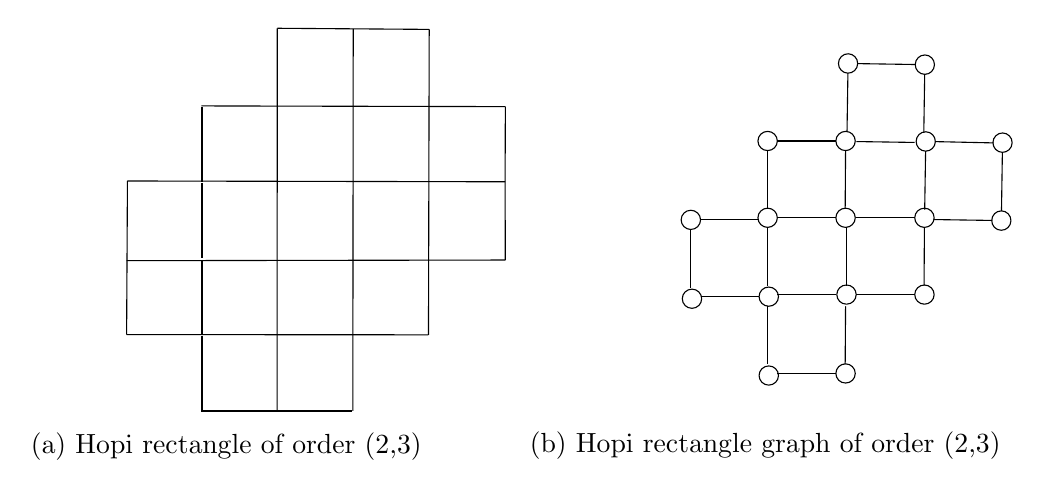
\begin{tikzpicture}[x=0.75pt,y=0.75pt,yscale=-1,xscale=1]
%uncomment if require: \path (0,3166); %set diagram left start at 0, and has height of 3166

%Shape: Ellipse [id:dp01904085319587523] 
\draw   (456.77,1593.93) .. controls (456.77,1591.37) and (458.86,1589.3) .. (461.44,1589.3) .. controls (464.02,1589.3) and (466.11,1591.37) .. (466.11,1593.93) .. controls (466.11,1596.48) and (464.02,1598.55) .. (461.44,1598.55) .. controls (458.86,1598.55) and (456.77,1596.48) .. (456.77,1593.93) -- cycle ;
%Shape: Ellipse [id:dp37159111248956744] 
\draw   (494.32,1593.93) .. controls (494.32,1591.37) and (496.41,1589.3) .. (498.99,1589.3) .. controls (501.57,1589.3) and (503.66,1591.37) .. (503.66,1593.93) .. controls (503.66,1596.48) and (501.57,1598.55) .. (498.99,1598.55) .. controls (496.41,1598.55) and (494.32,1596.48) .. (494.32,1593.93) -- cycle ;
%Straight Lines [id:da9581124404097807] 
\draw    (466.11,1593.93) -- (494.32,1593.93) ;
%Straight Lines [id:da8023645165409672] 
\draw    (461.44,1598.55) -- (461.44,1626.59) ;
%Straight Lines [id:da5512003550437814] 
\draw    (498.99,1598.55) -- (498.8,1626.59) ;
%Shape: Ellipse [id:dp1889931077399356] 
\draw   (456.77,1630.93) .. controls (456.77,1628.37) and (458.86,1626.3) .. (461.44,1626.3) .. controls (464.02,1626.3) and (466.11,1628.37) .. (466.11,1630.93) .. controls (466.11,1633.48) and (464.02,1635.55) .. (461.44,1635.55) .. controls (458.86,1635.55) and (456.77,1633.48) .. (456.77,1630.93) -- cycle ;
%Shape: Ellipse [id:dp8143048313704453] 
\draw   (494.32,1630.93) .. controls (494.32,1628.37) and (496.41,1626.3) .. (498.99,1626.3) .. controls (501.57,1626.3) and (503.66,1628.37) .. (503.66,1630.93) .. controls (503.66,1633.48) and (501.57,1635.55) .. (498.99,1635.55) .. controls (496.41,1635.55) and (494.32,1633.48) .. (494.32,1630.93) -- cycle ;
%Straight Lines [id:da49225027769716134] 
\draw    (466.11,1630.93) -- (494.32,1630.93) ;
%Shape: Ellipse [id:dp8912304799504929] 
\draw   (532.32,1630.93) .. controls (532.32,1628.37) and (534.41,1626.3) .. (536.99,1626.3) .. controls (539.57,1626.3) and (541.66,1628.37) .. (541.66,1630.93) .. controls (541.66,1633.48) and (539.57,1635.55) .. (536.99,1635.55) .. controls (534.41,1635.55) and (532.32,1633.48) .. (532.32,1630.93) -- cycle ;
%Straight Lines [id:da2381813614606989] 
\draw    (504.11,1630.93) -- (532.32,1630.93) ;
%Straight Lines [id:da9222015388292022] 
\draw    (499.44,1635.55) -- (499.44,1663.59) ;
%Straight Lines [id:da05653010242664691] 
\draw    (536.99,1635.55) -- (536.8,1663.59) ;
%Shape: Ellipse [id:dp35291465754070517] 
\draw   (494.77,1667.93) .. controls (494.77,1665.37) and (496.86,1663.3) .. (499.44,1663.3) .. controls (502.02,1663.3) and (504.11,1665.37) .. (504.11,1667.93) .. controls (504.11,1670.48) and (502.02,1672.55) .. (499.44,1672.55) .. controls (496.86,1672.55) and (494.77,1670.48) .. (494.77,1667.93) -- cycle ;
%Shape: Ellipse [id:dp5543350995441292] 
\draw   (532.32,1667.93) .. controls (532.32,1665.37) and (534.41,1663.3) .. (536.99,1663.3) .. controls (539.57,1663.3) and (541.66,1665.37) .. (541.66,1667.93) .. controls (541.66,1670.48) and (539.57,1672.55) .. (536.99,1672.55) .. controls (534.41,1672.55) and (532.32,1670.48) .. (532.32,1667.93) -- cycle ;
%Straight Lines [id:da3320441854608036] 
\draw    (504.11,1667.93) -- (532.32,1667.93) ;
%Shape: Ellipse [id:dp3679335748583392] 
\draw   (537.55,1598.83) .. controls (534.99,1598.79) and (532.95,1596.67) .. (532.99,1594.09) .. controls (533.03,1591.51) and (535.13,1589.45) .. (537.69,1589.49) .. controls (540.24,1589.53) and (542.28,1591.65) .. (542.24,1594.23) .. controls (542.2,1596.81) and (540.1,1598.87) .. (537.55,1598.83) -- cycle ;
%Straight Lines [id:da9515324089121131] 
\draw    (537.11,1627.04) -- (537.55,1598.83) ;
%Straight Lines [id:da09090527653917713] 
\draw    (541.67,1631.78) -- (569.7,1632.21) ;
%Straight Lines [id:da8989646448477504] 
\draw    (542.24,1594.23) -- (570.28,1594.85) ;
%Shape: Ellipse [id:dp2944149646093772] 
\draw   (573.96,1636.94) .. controls (571.41,1636.91) and (569.37,1634.78) .. (569.41,1632.2) .. controls (569.45,1629.62) and (571.55,1627.57) .. (574.11,1627.6) .. controls (576.66,1627.64) and (578.7,1629.77) .. (578.66,1632.35) .. controls (578.62,1634.93) and (576.52,1636.98) .. (573.96,1636.94) -- cycle ;
%Shape: Ellipse [id:dp20356554974707497] 
\draw   (574.54,1599.4) .. controls (571.99,1599.36) and (569.95,1597.23) .. (569.99,1594.66) .. controls (570.03,1592.08) and (572.13,1590.02) .. (574.68,1590.06) .. controls (577.24,1590.1) and (579.28,1592.22) .. (579.24,1594.8) .. controls (579.2,1597.38) and (577.1,1599.44) .. (574.54,1599.4) -- cycle ;
%Straight Lines [id:da11350481319187478] 
\draw    (574.11,1627.6) -- (574.54,1599.4) ;
%Shape: Ellipse [id:dp9881516134578121] 
\draw   (500.12,1561.25) .. controls (497.56,1561.21) and (495.52,1559.09) .. (495.56,1556.51) .. controls (495.6,1553.93) and (497.71,1551.87) .. (500.26,1551.91) .. controls (502.82,1551.95) and (504.86,1554.07) .. (504.82,1556.65) .. controls (504.78,1559.23) and (502.67,1561.29) .. (500.12,1561.25) -- cycle ;
%Straight Lines [id:da26909923805856084] 
\draw    (499.69,1589.46) -- (500.12,1561.25) ;
%Straight Lines [id:da49622962209931076] 
\draw    (504.24,1594.2) -- (532.27,1594.63) ;
%Straight Lines [id:da7534028269370452] 
\draw    (504.82,1556.65) -- (532.56,1557.08) ;
%Shape: Ellipse [id:dp8798846767837143] 
\draw   (537.11,1561.82) .. controls (534.56,1561.78) and (532.52,1559.66) .. (532.56,1557.08) .. controls (532.6,1554.5) and (534.7,1552.44) .. (537.26,1552.48) .. controls (539.81,1552.52) and (541.85,1554.64) .. (541.81,1557.22) .. controls (541.77,1559.8) and (539.67,1561.86) .. (537.11,1561.82) -- cycle ;
%Straight Lines [id:da8063536496900947] 
\draw    (536.68,1590.03) -- (537.11,1561.82) ;
%Straight Lines [id:da6606683005902503] 
\draw    (188.61,1577.03) -- (335.08,1577.37) ;
%Straight Lines [id:da45994481444788904] 
\draw    (188.94,1577.65) -- (188.94,1613.69) ;
%Straight Lines [id:da12909379613121907] 
\draw    (188.94,1614.15) -- (188.94,1650.19) ;
%Straight Lines [id:da7869808565297138] 
\draw    (188.94,1651.15) -- (188.94,1687.19) ;
%Straight Lines [id:da0199477540414168] 
\draw    (188.94,1687.65) -- (188.94,1723.69) ;
%Straight Lines [id:da7925707095899002] 
\draw    (188.61,1724.03) -- (224.82,1724.03) ;
%Straight Lines [id:da13419442850900865] 
\draw    (225.11,1724.03) -- (261.32,1724.03) ;
%Straight Lines [id:da8403535726203732] 
\draw    (152.6,1687.2) -- (298.04,1687.32) ;
%Straight Lines [id:da16560771064141866] 
\draw    (152.6,1651.6) -- (335.05,1651.28) ;
%Straight Lines [id:da7253157221313775] 
\draw    (152.6,1687.2) -- (153,1613.2) ;
%Straight Lines [id:da2730541034499703] 
\draw    (153,1613.2) -- (334.95,1613.58) ;
%Shape: Ellipse [id:dp8937276195771653] 
\draw   (457.32,1668.93) .. controls (457.32,1666.37) and (459.41,1664.3) .. (461.99,1664.3) .. controls (464.57,1664.3) and (466.66,1666.37) .. (466.66,1668.93) .. controls (466.66,1671.48) and (464.57,1673.55) .. (461.99,1673.55) .. controls (459.41,1673.55) and (457.32,1671.48) .. (457.32,1668.93) -- cycle ;
%Straight Lines [id:da3947073995717243] 
\draw    (461.44,1635.55) -- (461.44,1663.59) ;
%Straight Lines [id:da2620728627863276] 
\draw    (466.11,1667.93) -- (494.32,1667.93) ;
%Shape: Ellipse [id:dp7049269965027793] 
\draw   (420.32,1669.93) .. controls (420.32,1667.37) and (422.41,1665.3) .. (424.99,1665.3) .. controls (427.57,1665.3) and (429.66,1667.37) .. (429.66,1669.93) .. controls (429.66,1672.48) and (427.57,1674.55) .. (424.99,1674.55) .. controls (422.41,1674.55) and (420.32,1672.48) .. (420.32,1669.93) -- cycle ;
%Shape: Ellipse [id:dp5715950498897249] 
\draw   (419.77,1631.93) .. controls (419.77,1629.37) and (421.86,1627.3) .. (424.44,1627.3) .. controls (427.02,1627.3) and (429.11,1629.37) .. (429.11,1631.93) .. controls (429.11,1634.48) and (427.02,1636.55) .. (424.44,1636.55) .. controls (421.86,1636.55) and (419.77,1634.48) .. (419.77,1631.93) -- cycle ;
%Straight Lines [id:da10340562293058508] 
\draw    (429.11,1631.93) -- (457.32,1631.93) ;
%Straight Lines [id:da06745250216058274] 
\draw    (424.44,1636.55) -- (424.44,1664.59) ;
%Straight Lines [id:da27600709236179655] 
\draw    (429.11,1668.93) -- (457.32,1668.93) ;
%Shape: Ellipse [id:dp7217942064022724] 
\draw   (457.32,1706.93) .. controls (457.32,1704.37) and (459.41,1702.3) .. (461.99,1702.3) .. controls (464.57,1702.3) and (466.66,1704.37) .. (466.66,1706.93) .. controls (466.66,1709.48) and (464.57,1711.55) .. (461.99,1711.55) .. controls (459.41,1711.55) and (457.32,1709.48) .. (457.32,1706.93) -- cycle ;
%Straight Lines [id:da4374133080546154] 
\draw    (461.44,1673.55) -- (461.44,1701.59) ;
%Straight Lines [id:da9672309312187011] 
\draw    (498.99,1673.55) -- (498.8,1701.59) ;
%Shape: Ellipse [id:dp29420624078095425] 
\draw   (494.32,1705.93) .. controls (494.32,1703.37) and (496.41,1701.3) .. (498.99,1701.3) .. controls (501.57,1701.3) and (503.66,1703.37) .. (503.66,1705.93) .. controls (503.66,1708.48) and (501.57,1710.55) .. (498.99,1710.55) .. controls (496.41,1710.55) and (494.32,1708.48) .. (494.32,1705.93) -- cycle ;
%Straight Lines [id:da19852907123271657] 
\draw    (466.11,1705.93) -- (494.32,1705.93) ;
%Straight Lines [id:da8695189800128807] 
\draw    (225.18,1539.62) -- (225.11,1724.03) ;
%Straight Lines [id:da22606257599411872] 
\draw    (261.78,1539.89) -- (261.59,1723.93) ;
%Straight Lines [id:da6831060045408865] 
\draw    (298.39,1540.16) -- (298.04,1687.32) ;
%Straight Lines [id:da006281760138264314] 
\draw    (225.18,1539.62) -- (298.39,1540.16) ;
%Straight Lines [id:da7575848704289305] 
\draw    (335.08,1577.37) -- (334.95,1613.58) ;
%Straight Lines [id:da9094189281464261] 
\draw    (334.95,1613.58) -- (335.05,1651.28) ;

% Text Node
\draw (105.2,1733.4) node [anchor=north west][inner sep=0.75pt]  [font=\normalsize] [align=left] {(a) Hopi rectangle of order (2,3)};
% Text Node
\draw (345.6,1732.6) node [anchor=north west][inner sep=0.75pt]   [align=left] {(b) Hopi rectangle graph of order (2,3)};


\end{tikzpicture}
    \caption{}
    \label{fig:Ad&ADgraph}
\end{figure}





In \cite{KnuthAztecDiamond}, the authors defined the \textit{Hopi diamond graph of order $n$} as a graph on $nm$ vertices. Later \cite{VisualDefAztecDiamond} offered a more visual perspective on these graphs. This visual approach provided a useful foundation for working with the graph family and motivated our formulation of the Hopi rectangle graph in Definition \ref{def:UpdatedDefAD_{m,n}}. Our definition views the Hopi rectangle graph of order $(a,b)$ as an induced subgraph of the 2-dimensional grid graph $P_{a+b}\square P_{a+b}$ and was necessary both for implementing our work in SageMath, particularly in applying the algorithm described in \cite{moruzziLeakyForcing}, and for establishing several of our results by viewing the graph as being embedded in an integer lattice. Our definition, presented below, is motivated both by the visual formulation and by the techniques found in \cite{TechniquesLowerBoundZF}.


\begin{defn}\label{def:UpdatedDefAD_{m,n}}
    Let $a,b \in \mathbb{N}$ and consider the 2-dimensional grid graph given by $P_{a+b} \square P_{a+b}$. The \textit{Hopi rectangle graph of order $(a,b)$}, denoted by $HD(a,b)$, is the induced subgraph of $P_{a+b}\square P_{a+b}$ determined by the following subset of vertices
    $$H = \{(i,j): a-1 \leq i+j \leq 2b+a-1 \text{ and } |i-j| \leq a\}.$$

    \noindent That is, $HD(a,b) := (P_{a+b}\square P_{a+b})[H]$.
    %  The edge set of $HD(a,b)$ is given by the corresponding edges of $P_{a+b} \square P_{a+b}$. That is, for vertices
    % $(i,j),(i',j')\in V(HD(a,b))$:
    % $$E(HD(a,b))=\{(i,j)\sim(i',j'): i = i' \text{ and }  j\sim j' \in E(P_{a+b}) \text{ or }
    % j=j' \text{ and } i\sim i' \in E(P_{a+b})\}$$ 

\end{defn} 

Visually, from our definition, starting with the 2-dimensional grid graph $P_{a+b} \square P_{a+b}$, we can construct $HD(a,b)$ by removing vertices from the corners according to the following conditions. Vertices with $i+j < a-1$ are removed from the lower-left corner, while those with $i+j > 2b+a-1$ are removed from the upper-right corner. The restriction $|i-j| \leq a$ excludes the upper-left and lower-right corners. We note that under this indexing convention, the vertex of $HD(a,b)$ with the largest $j$-coordinate is $(b, a+b-1)$.

% Owing to the construction of the Hopi rectangle graph of order $(m,n)$, we have the following observation, which highlights the symmetry of this graph family and will be used in subsequent sections.
% \begin{obs}\label{obs:IsomorphicAsGraphs}
% For all $m,n \in \mathbb{N}$, $HD(m,n) \cong HD(n,m)$ as graphs.
% \end{obs}

Because of the high structure of this graph family, the number of vertices of a Hopi rectangle graph $HD(a,b)$ is given in the following proposition, which can be shown with an induction on $a$ and $b$. 

\begin{prop}\label{prop: Order of HD(m,n)}
For any $a,b \in \mathbb{N}$, the order of the Hopi rectangle graph of order $(a,b)$ is given by 
\[|V(HD(a,b))| = a+b + 2ab \] 
\end{prop}

It is a known observation that if an edge covering of a graph $G$ is determined by a set of subgraphs $H_i$, then the minimum rank of the graph $G$ is bounded above (and hence the maximum nullity bounded below) by the sum of the minimum ranks of the subgraphs $H_i$ which compose its edge covering \cite{FallatHogbenObservation}. That is,
\begin{equation}\label{eq:lowerboundmr}
    \text{mr}(G)\leq \sum_{i=1}^h \text{mr}(H_i),
\end{equation}

\noindent where $E(G) = \cup_i E(H_i)$. Utilizing this observation, we have the following two propositions that will be useful in establishing a lower bound on the maximum nullity of a given Hopi rectangle graph.


\begin{prop}\label{prop:edgecoverbounds}
    Let $G$ be any graph. If $G$ admits an edge covering by $\alpha$ copies of the cycle graph $C_4$, then $M(G) \ge |V(G)| - 2\cdot \alpha$.
\end{prop}

\begin{proof}
Let $G$ be a graph that admits an edge covering by $\alpha$ copies of $C_4$. By equation \ref{eq:lowerboundmr}, we have \[M(G) = |V(G)| - \operatorname{mr}(G) \ge |V(G)|  - \sum\limits_{i=1}^\alpha \operatorname{mr}(C_4).\] Since $\operatorname{mr}(C_4) = 2$, the result follows.
\end{proof}

\begin{prop}\label{prop:Edge Cover HD(m,n)}
For any $a,b\in\mathbb{N}$, there is an edge covering of the Hopi rectangle graph of order $(a,b)$ determined by $a\cdot b$ copies of the cycle subgraph $C_4$. In particular, $E(HD(a,b)) = \bigcup\limits_{i=1}^{ab} E((C_4))$.                                 
\end{prop}

\begin{proof}
	Consider the Hopi rectangle graph of order $(a,b)$, $HD(a,b)$. Proceeding with induction on $a$, consider $HD(1,b)$. We see that we can cover the edges of $HD(1,b)$ with $b$ copies of $C_4$ and write $E(HD(1,b)) = \bigcup\limits_{i=1}^{b} E((C_4))$. Now, suppose the edges of the graph $HD(a,b)$ can be covered via $a\cdot b$ copies of $C_4$, that is, $E(HD(a,b)) = \bigcup\limits_{i=1}^{ab} E((C_4))$. Considering $HD(a+1,b)$, one way to construct this graph is to begin with $HD(a,b)$ and adjoin $HD(1,b)$. This can be done by overlapping the degree two vertices along the upper boundary of $HD(1,b)$ with the degree two vertices along the lower boundary of $HD(a,b)$. Thus, accounting for all edges, we get that $E(HD(a+1,b)) =  E(HD(a,b)) \cup E(HD(1,b))$ as sets of edges and
        $$E(HD(a+1,b)) = \bigcup\limits_{i=1}^{ab} E((C_4)) \cup \bigcup\limits_{i=1}^{b} E((C_4)) = \bigcup\limits_{i=1}^{(a+1)b} E((C_4)),$$ 
    as desired.
\end{proof}



Combining Proposition \ref{prop:edgecoverbounds} and Proposition \ref{prop:Edge Cover HD(m,n)}, we get an upper bound on the minimum rank of $HD(a,b)$ and subsequently a lower bound on the maximum nullity of $HD(a,b)$. 



\begin{cor}\label{cor:Min Rank HD(m,n)}
    The minimum rank of the Hopi Rectangle graph $HD(a,b)$ of order $(a,b)$ is bounded above by $2ab$, i.e. $$\text{mr}(HD(a,b))\leq 2ab.$$
Moreover, the maximum nullity of $HD(a,b)$ is bounded below by $a+b$. 
\end{cor}

% \begin{proof}
%     We note that the graph $HD(m,n)$ admits an edge covering of $mn$ copies of $C_4$. Thus, we get \[ M(HD(m,n) \ge |V(HD(m,n))| - 2m n\]
%     The second part follows by a direct application of the rank-nullity theorem together with the order of $HD(m,n)$ given in Proposition \ref{prop: Order of HD(m,n)}.
% \end{proof}





\section{Zero forcing and leaky forcing on Hopi rectangle graphs}\label{sec:ZFonHopiRectanlges}
We now determine the zero forcing number and the leaky forcing numbers for the family of induced subgraphs \(HD(a,b)\) of \(P_{a+b}\square P_{a+b}\). In particular, our computation of the zero forcing number also shows that, for this family, maximum nullity and zero forcing coincide. We then turn to determining the leaky forcing numbers for this graph family. For \(\ell\ge 2\), we apply the results of Section~\ref{sec:FortsInducedSubgraphs} to fully characterize \(Z_{(\ell)}(HD(a,b))\). For \(\ell=1\), we instead use Theorem~\ref{prop:twoways} to determine \(Z_{(1)}(HD(a,b))\). Taken together, these cases suggest that a focused study of \(1\)-leaky forcing in induced subgraphs of \(d\)-dimensional grids would be a natural direction for future work.



\begin{lem}\label{lem:ZF Upper Bound}
Let $a,b \in \mathbb{N}$ and consider the following subset of vertices of $HD(a,b)$ 
\begin{equation}\label{eq:ZeroForcingSet}
    B=\{(i,j): i+j=a-1\}\cup\{(i,j):j=i+a\} \subseteq V(HD(a,b)).
\end{equation}
Then, the set $B$ has cardinality $a+b$ and is a zero forcing set of $HD(a,b)$.
\end{lem}
\begin{proof} 
\noindent Let $B_1 = \{(i,j): i+j=a-1\}$, $B_2 =\{(i,j):j=i+a\} $ and $B= B_1 \cup B_2$. We can see that, on the 2-dimensional grid $P_{a+b}\square P_{a+b}$, we have $|B_1| = a$ integer lattice points $(i,j)\in V(HD(a,b))$ that satisfy $i+j = a-1$. Similarly, there are exactly $|B_2| = b$ integer lattice points $(i,j)\in V(HD(a,b))$ that satisfy $j=i+a$. Also, if there was a coordinate point $(i,j)\in B_1\cap B_2$, then that coordinate point would have to satisfy the equation $i+(i+a) = a-1$, i.e. $2i = -1$, which does not have an integer solution. Therefore, $B_1\cap B_2 = \emptyset$ and 
    $$|B| = |B_1| + |B_2| - |B_1\cap B_2| = a+b.$$

\noindent Furthermore, we can see this set forces the entire graph blue by forcing horizontally across the graph, examples of which can be seen in Figure \ref{fig:Zfexample}. Hence, by induction on the rounds of forcing, every vertex of $HD(a,b)$ is eventually colored blue.
\end{proof}

\begin{figure}[h!]
    \centering





\tikzset{every picture/.style={line width=0.75pt}} %set default line width to 0.75pt        

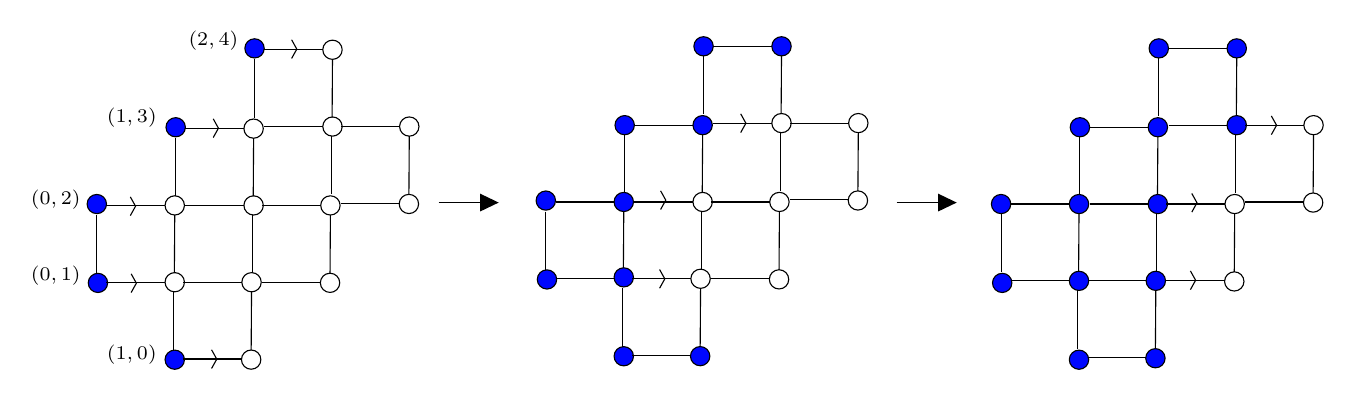
\begin{tikzpicture}[x=0.75pt,y=0.75pt,yscale=-1,xscale=1]
%uncomment if require: \path (0,274); %set diagram left start at 0, and has height of 274

%Shape: Ellipse [id:dp9766459966664965] 
\draw  [fill={rgb, 255:red, 0; green, 7; blue, 255 }  ,fill opacity=1 ] (47.25,177.37) .. controls (47.25,174.82) and (49.34,172.75) .. (51.92,172.75) .. controls (54.5,172.75) and (56.59,174.82) .. (56.59,177.37) .. controls (56.59,179.93) and (54.5,182) .. (51.92,182) .. controls (49.34,182) and (47.25,179.93) .. (47.25,177.37) -- cycle ;
%Shape: Ellipse [id:dp6589450851529929] 
\draw  [fill={rgb, 255:red, 0; green, 7; blue, 255 }  ,fill opacity=1 ] (46.7,139.37) .. controls (46.7,136.82) and (48.79,134.75) .. (51.37,134.75) .. controls (53.95,134.75) and (56.04,136.82) .. (56.04,139.37) .. controls (56.04,141.93) and (53.95,144) .. (51.37,144) .. controls (48.79,144) and (46.7,141.93) .. (46.7,139.37) -- cycle ;
%Shape: Ellipse [id:dp10758165828178401] 
\draw   (84.25,140.04) .. controls (84.25,137.48) and (86.34,135.41) .. (88.92,135.41) .. controls (91.5,135.41) and (93.59,137.48) .. (93.59,140.04) .. controls (93.59,142.6) and (91.5,144.67) .. (88.92,144.67) .. controls (86.34,144.67) and (84.25,142.6) .. (84.25,140.04) -- cycle ;
%Straight Lines [id:da38988268909461476] 
\draw    (56.04,140.04) -- (84.25,140.04) ;
%Straight Lines [id:da8885043061886748] 
\draw    (51.37,144.67) -- (51.37,172.71) ;
%Straight Lines [id:da29786636492509144] 
\draw    (88.92,144.67) -- (88.74,172.71) ;
%Shape: Ellipse [id:dp1712750401178178] 
\draw   (84.25,177.04) .. controls (84.25,174.48) and (86.34,172.41) .. (88.92,172.41) .. controls (91.5,172.41) and (93.59,174.48) .. (93.59,177.04) .. controls (93.59,179.6) and (91.5,181.67) .. (88.92,181.67) .. controls (86.34,181.67) and (84.25,179.6) .. (84.25,177.04) -- cycle ;
%Straight Lines [id:da04387905886133514] 
\draw    (56.04,177.04) -- (84.25,177.04) ;
%Shape: Ellipse [id:dp5334578932118021] 
\draw  [fill={rgb, 255:red, 0; green, 7; blue, 255 }  ,fill opacity=1 ] (84.25,214.37) .. controls (84.25,211.82) and (86.34,209.75) .. (88.92,209.75) .. controls (91.5,209.75) and (93.59,211.82) .. (93.59,214.37) .. controls (93.59,216.93) and (91.5,219) .. (88.92,219) .. controls (86.34,219) and (84.25,216.93) .. (84.25,214.37) -- cycle ;
%Shape: Ellipse [id:dp1550781947328569] 
\draw   (121.25,177.04) .. controls (121.25,174.48) and (123.34,172.41) .. (125.92,172.41) .. controls (128.5,172.41) and (130.59,174.48) .. (130.59,177.04) .. controls (130.59,179.6) and (128.5,181.67) .. (125.92,181.67) .. controls (123.34,181.67) and (121.25,179.6) .. (121.25,177.04) -- cycle ;
%Straight Lines [id:da02862337244794677] 
\draw    (93.04,177.04) -- (121.25,177.04) ;
%Straight Lines [id:da6723019172884572] 
\draw    (88.37,181.67) -- (88.37,209.71) ;
%Straight Lines [id:da3961607577895735] 
\draw    (125.92,181.67) -- (125.74,209.71) ;
%Shape: Ellipse [id:dp982137549971329] 
\draw   (121.07,214.33) .. controls (121.07,211.78) and (123.16,209.71) .. (125.74,209.71) .. controls (128.32,209.71) and (130.41,211.78) .. (130.41,214.33) .. controls (130.41,216.89) and (128.32,218.96) .. (125.74,218.96) .. controls (123.16,218.96) and (121.07,216.89) .. (121.07,214.33) -- cycle ;
%Straight Lines [id:da2637336220731491] 
\draw    (93.04,214.04) -- (121.25,214.04) ;
%Shape: Ellipse [id:dp6857086623342689] 
\draw  [fill={rgb, 255:red, 0; green, 7; blue, 255 }  ,fill opacity=1 ] (84.7,102.37) .. controls (84.7,99.82) and (86.79,97.75) .. (89.37,97.75) .. controls (91.95,97.75) and (94.04,99.82) .. (94.04,102.37) .. controls (94.04,104.93) and (91.95,107) .. (89.37,107) .. controls (86.79,107) and (84.7,104.93) .. (84.7,102.37) -- cycle ;
%Shape: Ellipse [id:dp3326898639669711] 
\draw   (122.25,103.04) .. controls (122.25,100.48) and (124.34,98.41) .. (126.92,98.41) .. controls (129.5,98.41) and (131.59,100.48) .. (131.59,103.04) .. controls (131.59,105.6) and (129.5,107.67) .. (126.92,107.67) .. controls (124.34,107.67) and (122.25,105.6) .. (122.25,103.04) -- cycle ;
%Straight Lines [id:da8167300357875875] 
\draw    (94.04,103.04) -- (122.25,103.04) ;
%Straight Lines [id:da3794742025321288] 
\draw    (89.37,107.67) -- (89.37,135.71) ;
%Straight Lines [id:da6908989906120665] 
\draw    (126.92,107.67) -- (126.74,135.71) ;
%Shape: Ellipse [id:dp21468385425091885] 
\draw   (122.25,140.04) .. controls (122.25,137.48) and (124.34,135.41) .. (126.92,135.41) .. controls (129.5,135.41) and (131.59,137.48) .. (131.59,140.04) .. controls (131.59,142.6) and (129.5,144.67) .. (126.92,144.67) .. controls (124.34,144.67) and (122.25,142.6) .. (122.25,140.04) -- cycle ;
%Straight Lines [id:da843877420814539] 
\draw    (94.04,140.04) -- (122.25,140.04) ;
%Shape: Ellipse [id:dp5484429851982529] 
\draw   (159.25,140.04) .. controls (159.25,137.48) and (161.34,135.41) .. (163.92,135.41) .. controls (166.5,135.41) and (168.59,137.48) .. (168.59,140.04) .. controls (168.59,142.6) and (166.5,144.67) .. (163.92,144.67) .. controls (161.34,144.67) and (159.25,142.6) .. (159.25,140.04) -- cycle ;
%Straight Lines [id:da8270885930324198] 
\draw    (131.04,140.04) -- (159.25,140.04) ;
%Straight Lines [id:da6158201586934898] 
\draw    (126.37,144.67) -- (126.37,172.71) ;
%Straight Lines [id:da7709393325035707] 
\draw    (163.92,144.67) -- (163.74,172.71) ;
%Shape: Ellipse [id:dp18584441306102129] 
\draw   (159.07,177.33) .. controls (159.07,174.78) and (161.16,172.71) .. (163.74,172.71) .. controls (166.32,172.71) and (168.41,174.78) .. (168.41,177.33) .. controls (168.41,179.89) and (166.32,181.96) .. (163.74,181.96) .. controls (161.16,181.96) and (159.07,179.89) .. (159.07,177.33) -- cycle ;
%Straight Lines [id:da5715872456152564] 
\draw    (131.04,177.04) -- (159.25,177.04) ;
%Shape: Ellipse [id:dp3078439786798889] 
\draw  [fill={rgb, 255:red, 0; green, 7; blue, 255 }  ,fill opacity=1 ] (122.7,64.37) .. controls (122.7,61.82) and (124.79,59.75) .. (127.37,59.75) .. controls (129.95,59.75) and (132.04,61.82) .. (132.04,64.37) .. controls (132.04,66.93) and (129.95,69) .. (127.37,69) .. controls (124.79,69) and (122.7,66.93) .. (122.7,64.37) -- cycle ;
%Shape: Ellipse [id:dp017713915108829248] 
\draw   (160.25,65.04) .. controls (160.25,62.48) and (162.34,60.41) .. (164.92,60.41) .. controls (167.5,60.41) and (169.59,62.48) .. (169.59,65.04) .. controls (169.59,67.6) and (167.5,69.67) .. (164.92,69.67) .. controls (162.34,69.67) and (160.25,67.6) .. (160.25,65.04) -- cycle ;
%Straight Lines [id:da17187573701785264] 
\draw    (132.04,65.04) -- (160.25,65.04) ;
%Straight Lines [id:da4347750718493423] 
\draw    (127.37,69.67) -- (127.37,97.71) ;
%Straight Lines [id:da9561639203022528] 
\draw    (164.92,69.67) -- (164.74,97.71) ;
%Shape: Ellipse [id:dp7381707718759748] 
\draw   (160.25,102.04) .. controls (160.25,99.48) and (162.34,97.41) .. (164.92,97.41) .. controls (167.5,97.41) and (169.59,99.48) .. (169.59,102.04) .. controls (169.59,104.6) and (167.5,106.67) .. (164.92,106.67) .. controls (162.34,106.67) and (160.25,104.6) .. (160.25,102.04) -- cycle ;
%Straight Lines [id:da33736669691152577] 
\draw    (132.04,102.04) -- (160.25,102.04) ;
%Shape: Ellipse [id:dp8674167331521759] 
\draw   (197.25,102.04) .. controls (197.25,99.48) and (199.34,97.41) .. (201.92,97.41) .. controls (204.5,97.41) and (206.59,99.48) .. (206.59,102.04) .. controls (206.59,104.6) and (204.5,106.67) .. (201.92,106.67) .. controls (199.34,106.67) and (197.25,104.6) .. (197.25,102.04) -- cycle ;
%Straight Lines [id:da5635253221035833] 
\draw    (169.04,102.04) -- (197.25,102.04) ;
%Straight Lines [id:da6031545196928294] 
\draw    (164.37,106.67) -- (164.37,134.71) ;
%Straight Lines [id:da0022074409986814203] 
\draw    (201.92,106.67) -- (201.74,134.71) ;
%Shape: Ellipse [id:dp23459872017557215] 
\draw   (197.07,139.33) .. controls (197.07,136.78) and (199.16,134.71) .. (201.74,134.71) .. controls (204.32,134.71) and (206.41,136.78) .. (206.41,139.33) .. controls (206.41,141.89) and (204.32,143.96) .. (201.74,143.96) .. controls (199.16,143.96) and (197.07,141.89) .. (197.07,139.33) -- cycle ;
%Straight Lines [id:da3412179318091588] 
\draw    (169.04,139.04) -- (197.25,139.04) ;
%Shape: Ellipse [id:dp5086994768337447] 
\draw  [fill={rgb, 255:red, 0; green, 7; blue, 255 }  ,fill opacity=1 ] (263.59,175.71) .. controls (263.59,173.15) and (265.68,171.08) .. (268.26,171.08) .. controls (270.84,171.08) and (272.93,173.15) .. (272.93,175.71) .. controls (272.93,178.26) and (270.84,180.33) .. (268.26,180.33) .. controls (265.68,180.33) and (263.59,178.26) .. (263.59,175.71) -- cycle ;
%Shape: Ellipse [id:dp10580861978368239] 
\draw  [fill={rgb, 255:red, 0; green, 7; blue, 255 }  ,fill opacity=1 ] (263.03,137.71) .. controls (263.03,135.15) and (265.12,133.08) .. (267.7,133.08) .. controls (270.28,133.08) and (272.37,135.15) .. (272.37,137.71) .. controls (272.37,140.26) and (270.28,142.33) .. (267.7,142.33) .. controls (265.12,142.33) and (263.03,140.26) .. (263.03,137.71) -- cycle ;
%Shape: Ellipse [id:dp0902932185509332] 
\draw  [fill={rgb, 255:red, 0; green, 7; blue, 255 }  ,fill opacity=1 ] (300.59,138.37) .. controls (300.59,135.82) and (302.68,133.75) .. (305.26,133.75) .. controls (307.84,133.75) and (309.93,135.82) .. (309.93,138.37) .. controls (309.93,140.93) and (307.84,143) .. (305.26,143) .. controls (302.68,143) and (300.59,140.93) .. (300.59,138.37) -- cycle ;
%Straight Lines [id:da011207184814696403] 
\draw    (272.37,138.37) -- (300.59,138.37) ;
%Straight Lines [id:da4738768328697617] 
\draw    (267.7,143) -- (267.7,171.04) ;
%Straight Lines [id:da9004067779679389] 
\draw    (305.26,143) -- (305.07,171.04) ;
%Shape: Ellipse [id:dp4215997783098625] 
\draw  [fill={rgb, 255:red, 0; green, 7; blue, 255 }  ,fill opacity=1 ] (300.59,174.71) .. controls (300.59,172.15) and (302.68,170.08) .. (305.26,170.08) .. controls (307.84,170.08) and (309.93,172.15) .. (309.93,174.71) .. controls (309.93,177.26) and (307.84,179.33) .. (305.26,179.33) .. controls (302.68,179.33) and (300.59,177.26) .. (300.59,174.71) -- cycle ;
%Straight Lines [id:da6071610813811272] 
\draw    (272.37,175.37) -- (300.59,175.37) ;
%Shape: Ellipse [id:dp6543404995707597] 
\draw  [fill={rgb, 255:red, 0; green, 7; blue, 255 }  ,fill opacity=1 ] (300.59,212.71) .. controls (300.59,210.15) and (302.68,208.08) .. (305.26,208.08) .. controls (307.84,208.08) and (309.93,210.15) .. (309.93,212.71) .. controls (309.93,215.26) and (307.84,217.33) .. (305.26,217.33) .. controls (302.68,217.33) and (300.59,215.26) .. (300.59,212.71) -- cycle ;
%Shape: Ellipse [id:dp48065051821663307] 
\draw   (337.59,175.37) .. controls (337.59,172.82) and (339.68,170.75) .. (342.26,170.75) .. controls (344.84,170.75) and (346.93,172.82) .. (346.93,175.37) .. controls (346.93,177.93) and (344.84,180) .. (342.26,180) .. controls (339.68,180) and (337.59,177.93) .. (337.59,175.37) -- cycle ;
%Straight Lines [id:da7911560079021986] 
\draw    (309.37,175.37) -- (337.59,175.37) ;
%Straight Lines [id:da0799561820663901] 
\draw    (304.7,180) -- (304.7,208.04) ;
%Straight Lines [id:da41365096882235597] 
\draw    (342.26,180) -- (342.07,208.04) ;
%Shape: Ellipse [id:dp23405224146270864] 
\draw  [fill={rgb, 255:red, 0; green, 7; blue, 255 }  ,fill opacity=1 ] (337.4,212.67) .. controls (337.4,210.11) and (339.49,208.04) .. (342.07,208.04) .. controls (344.65,208.04) and (346.74,210.11) .. (346.74,212.67) .. controls (346.74,215.22) and (344.65,217.29) .. (342.07,217.29) .. controls (339.49,217.29) and (337.4,215.22) .. (337.4,212.67) -- cycle ;
%Straight Lines [id:da9499690873328616] 
\draw    (309.37,212.37) -- (337.59,212.37) ;
%Shape: Ellipse [id:dp20618268133961404] 
\draw  [fill={rgb, 255:red, 0; green, 7; blue, 255 }  ,fill opacity=1 ] (301.03,101.37) .. controls (301.03,98.82) and (303.12,96.75) .. (305.7,96.75) .. controls (308.28,96.75) and (310.37,98.82) .. (310.37,101.37) .. controls (310.37,103.93) and (308.28,106) .. (305.7,106) .. controls (303.12,106) and (301.03,103.93) .. (301.03,101.37) -- cycle ;
%Shape: Ellipse [id:dp04800600181436243] 
\draw  [fill={rgb, 255:red, 0; green, 7; blue, 255 }  ,fill opacity=1 ] (338.59,101.37) .. controls (338.59,98.82) and (340.68,96.75) .. (343.26,96.75) .. controls (345.84,96.75) and (347.93,98.82) .. (347.93,101.37) .. controls (347.93,103.93) and (345.84,106) .. (343.26,106) .. controls (340.68,106) and (338.59,103.93) .. (338.59,101.37) -- cycle ;
%Straight Lines [id:da1454073409443264] 
\draw    (310.37,101.37) -- (338.59,101.37) ;
%Straight Lines [id:da8168909581182984] 
\draw    (305.7,106) -- (305.7,134.04) ;
%Straight Lines [id:da8689576306025383] 
\draw    (343.26,106) -- (343.07,134.04) ;
%Shape: Ellipse [id:dp020807460389216104] 
\draw   (338.59,138.37) .. controls (338.59,135.82) and (340.68,133.75) .. (343.26,133.75) .. controls (345.84,133.75) and (347.93,135.82) .. (347.93,138.37) .. controls (347.93,140.93) and (345.84,143) .. (343.26,143) .. controls (340.68,143) and (338.59,140.93) .. (338.59,138.37) -- cycle ;
%Straight Lines [id:da5990507015874904] 
\draw    (310.37,138.37) -- (338.59,138.37) ;
%Shape: Ellipse [id:dp20918141995913708] 
\draw   (375.59,138.37) .. controls (375.59,135.82) and (377.68,133.75) .. (380.26,133.75) .. controls (382.84,133.75) and (384.93,135.82) .. (384.93,138.37) .. controls (384.93,140.93) and (382.84,143) .. (380.26,143) .. controls (377.68,143) and (375.59,140.93) .. (375.59,138.37) -- cycle ;
%Straight Lines [id:da11459369093012017] 
\draw    (347.37,138.37) -- (375.59,138.37) ;
%Straight Lines [id:da10062237987580713] 
\draw    (342.7,143) -- (342.7,171.04) ;
%Straight Lines [id:da5550604997239162] 
\draw    (380.26,143) -- (380.07,171.04) ;
%Shape: Ellipse [id:dp9031605111034653] 
\draw   (375.4,175.67) .. controls (375.4,173.11) and (377.49,171.04) .. (380.07,171.04) .. controls (382.65,171.04) and (384.74,173.11) .. (384.74,175.67) .. controls (384.74,178.22) and (382.65,180.29) .. (380.07,180.29) .. controls (377.49,180.29) and (375.4,178.22) .. (375.4,175.67) -- cycle ;
%Straight Lines [id:da7820707372350887] 
\draw    (347.37,175.37) -- (375.59,175.37) ;
%Shape: Ellipse [id:dp37700794417643546] 
\draw  [fill={rgb, 255:red, 0; green, 7; blue, 255 }  ,fill opacity=1 ] (339.03,63.37) .. controls (339.03,60.82) and (341.12,58.75) .. (343.7,58.75) .. controls (346.28,58.75) and (348.37,60.82) .. (348.37,63.37) .. controls (348.37,65.93) and (346.28,68) .. (343.7,68) .. controls (341.12,68) and (339.03,65.93) .. (339.03,63.37) -- cycle ;
%Shape: Ellipse [id:dp4987018521383706] 
\draw  [fill={rgb, 255:red, 0; green, 7; blue, 255 }  ,fill opacity=1 ] (376.59,63.37) .. controls (376.59,60.82) and (378.68,58.75) .. (381.26,58.75) .. controls (383.84,58.75) and (385.93,60.82) .. (385.93,63.37) .. controls (385.93,65.93) and (383.84,68) .. (381.26,68) .. controls (378.68,68) and (376.59,65.93) .. (376.59,63.37) -- cycle ;
%Straight Lines [id:da2738908956301823] 
\draw    (348.37,63.37) -- (376.59,63.37) ;
%Straight Lines [id:da3759943956674314] 
\draw    (343.7,68) -- (343.7,96.04) ;
%Straight Lines [id:da5037384002017504] 
\draw    (381.26,68) -- (381.07,96.04) ;
%Shape: Ellipse [id:dp5422176560235696] 
\draw   (376.59,100.37) .. controls (376.59,97.82) and (378.68,95.75) .. (381.26,95.75) .. controls (383.84,95.75) and (385.93,97.82) .. (385.93,100.37) .. controls (385.93,102.93) and (383.84,105) .. (381.26,105) .. controls (378.68,105) and (376.59,102.93) .. (376.59,100.37) -- cycle ;
%Straight Lines [id:da047811010600382176] 
\draw    (348.37,100.37) -- (376.59,100.37) ;
%Shape: Ellipse [id:dp14060845769037456] 
\draw   (413.59,100.37) .. controls (413.59,97.82) and (415.68,95.75) .. (418.26,95.75) .. controls (420.84,95.75) and (422.93,97.82) .. (422.93,100.37) .. controls (422.93,102.93) and (420.84,105) .. (418.26,105) .. controls (415.68,105) and (413.59,102.93) .. (413.59,100.37) -- cycle ;
%Straight Lines [id:da0523179957029033] 
\draw    (385.37,100.37) -- (413.59,100.37) ;
%Straight Lines [id:da6434089522272378] 
\draw    (380.7,105) -- (380.7,133.04) ;
%Straight Lines [id:da18030888811287138] 
\draw    (418.26,105) -- (418.07,133.04) ;
%Shape: Ellipse [id:dp06039735207823815] 
\draw   (413.4,137.67) .. controls (413.4,135.11) and (415.49,133.04) .. (418.07,133.04) .. controls (420.65,133.04) and (422.74,135.11) .. (422.74,137.67) .. controls (422.74,140.22) and (420.65,142.29) .. (418.07,142.29) .. controls (415.49,142.29) and (413.4,140.22) .. (413.4,137.67) -- cycle ;
%Straight Lines [id:da4311615382221333] 
\draw    (385.37,137.37) -- (413.59,137.37) ;
%Shape: Ellipse [id:dp08334274881983517] 
\draw  [fill={rgb, 255:red, 0; green, 7; blue, 255 }  ,fill opacity=1 ] (482.92,177.37) .. controls (482.92,174.82) and (485.01,172.75) .. (487.59,172.75) .. controls (490.17,172.75) and (492.26,174.82) .. (492.26,177.37) .. controls (492.26,179.93) and (490.17,182) .. (487.59,182) .. controls (485.01,182) and (482.92,179.93) .. (482.92,177.37) -- cycle ;
%Shape: Ellipse [id:dp33836248737783825] 
\draw  [fill={rgb, 255:red, 0; green, 7; blue, 255 }  ,fill opacity=1 ] (482.37,139.37) .. controls (482.37,136.82) and (484.46,134.75) .. (487.04,134.75) .. controls (489.62,134.75) and (491.71,136.82) .. (491.71,139.37) .. controls (491.71,141.93) and (489.62,144) .. (487.04,144) .. controls (484.46,144) and (482.37,141.93) .. (482.37,139.37) -- cycle ;
%Shape: Ellipse [id:dp5480571121881564] 
\draw  [fill={rgb, 255:red, 0; green, 7; blue, 255 }  ,fill opacity=1 ] (519.92,139.37) .. controls (519.92,136.82) and (522.01,134.75) .. (524.59,134.75) .. controls (527.17,134.75) and (529.26,136.82) .. (529.26,139.37) .. controls (529.26,141.93) and (527.17,144) .. (524.59,144) .. controls (522.01,144) and (519.92,141.93) .. (519.92,139.37) -- cycle ;
%Straight Lines [id:da7294285590545815] 
\draw    (491.71,139.37) -- (519.92,139.37) ;
%Straight Lines [id:da3382147055451157] 
\draw    (487.04,144) -- (487.04,172.04) ;
%Straight Lines [id:da3588494130342841] 
\draw    (524.59,144) -- (524.4,172.04) ;
%Shape: Ellipse [id:dp42574547231970683] 
\draw  [fill={rgb, 255:red, 0; green, 7; blue, 255 }  ,fill opacity=1 ] (519.92,176.37) .. controls (519.92,173.82) and (522.01,171.75) .. (524.59,171.75) .. controls (527.17,171.75) and (529.26,173.82) .. (529.26,176.37) .. controls (529.26,178.93) and (527.17,181) .. (524.59,181) .. controls (522.01,181) and (519.92,178.93) .. (519.92,176.37) -- cycle ;
%Straight Lines [id:da11319978915245255] 
\draw    (491.71,176.37) -- (519.92,176.37) ;
%Shape: Ellipse [id:dp5586998020455008] 
\draw  [fill={rgb, 255:red, 0; green, 7; blue, 255 }  ,fill opacity=1 ] (519.92,214.37) .. controls (519.92,211.82) and (522.01,209.75) .. (524.59,209.75) .. controls (527.17,209.75) and (529.26,211.82) .. (529.26,214.37) .. controls (529.26,216.93) and (527.17,219) .. (524.59,219) .. controls (522.01,219) and (519.92,216.93) .. (519.92,214.37) -- cycle ;
%Shape: Ellipse [id:dp7914709428752424] 
\draw  [fill={rgb, 255:red, 0; green, 7; blue, 255 }  ,fill opacity=1 ] (556.92,176.37) .. controls (556.92,173.82) and (559.01,171.75) .. (561.59,171.75) .. controls (564.17,171.75) and (566.26,173.82) .. (566.26,176.37) .. controls (566.26,178.93) and (564.17,181) .. (561.59,181) .. controls (559.01,181) and (556.92,178.93) .. (556.92,176.37) -- cycle ;
%Straight Lines [id:da09768255569745099] 
\draw    (528.71,176.37) -- (556.92,176.37) ;
%Straight Lines [id:da786362161589543] 
\draw    (524.04,181) -- (524.04,209.04) ;
%Straight Lines [id:da3604820102305619] 
\draw    (561.59,181) -- (561.4,209.04) ;
%Shape: Ellipse [id:dp3635549437314096] 
\draw  [fill={rgb, 255:red, 0; green, 7; blue, 255 }  ,fill opacity=1 ] (556.73,213.67) .. controls (556.73,211.11) and (558.82,209.04) .. (561.4,209.04) .. controls (563.98,209.04) and (566.07,211.11) .. (566.07,213.67) .. controls (566.07,216.22) and (563.98,218.29) .. (561.4,218.29) .. controls (558.82,218.29) and (556.73,216.22) .. (556.73,213.67) -- cycle ;
%Straight Lines [id:da1546485960545797] 
\draw    (528.71,213.37) -- (556.92,213.37) ;
%Shape: Ellipse [id:dp9952790973058048] 
\draw  [fill={rgb, 255:red, 0; green, 7; blue, 255 }  ,fill opacity=1 ] (520.37,102.37) .. controls (520.37,99.82) and (522.46,97.75) .. (525.04,97.75) .. controls (527.62,97.75) and (529.71,99.82) .. (529.71,102.37) .. controls (529.71,104.93) and (527.62,107) .. (525.04,107) .. controls (522.46,107) and (520.37,104.93) .. (520.37,102.37) -- cycle ;
%Shape: Ellipse [id:dp38331158881225724] 
\draw  [fill={rgb, 255:red, 0; green, 7; blue, 255 }  ,fill opacity=1 ] (557.92,102.37) .. controls (557.92,99.82) and (560.01,97.75) .. (562.59,97.75) .. controls (565.17,97.75) and (567.26,99.82) .. (567.26,102.37) .. controls (567.26,104.93) and (565.17,107) .. (562.59,107) .. controls (560.01,107) and (557.92,104.93) .. (557.92,102.37) -- cycle ;
%Straight Lines [id:da4093573252425534] 
\draw    (529.71,102.37) -- (557.92,102.37) ;
%Straight Lines [id:da4691931731970814] 
\draw    (525.04,107) -- (525.04,135.04) ;
%Straight Lines [id:da8527930813182659] 
\draw    (562.59,107) -- (562.4,135.04) ;
%Shape: Ellipse [id:dp9931393230847283] 
\draw  [fill={rgb, 255:red, 0; green, 7; blue, 255 }  ,fill opacity=1 ] (557.92,139.37) .. controls (557.92,136.82) and (560.01,134.75) .. (562.59,134.75) .. controls (565.17,134.75) and (567.26,136.82) .. (567.26,139.37) .. controls (567.26,141.93) and (565.17,144) .. (562.59,144) .. controls (560.01,144) and (557.92,141.93) .. (557.92,139.37) -- cycle ;
%Straight Lines [id:da2689837758577719] 
\draw    (529.71,139.37) -- (557.92,139.37) ;
%Shape: Ellipse [id:dp7484519260994427] 
\draw   (594.92,139.37) .. controls (594.92,136.82) and (597.01,134.75) .. (599.59,134.75) .. controls (602.17,134.75) and (604.26,136.82) .. (604.26,139.37) .. controls (604.26,141.93) and (602.17,144) .. (599.59,144) .. controls (597.01,144) and (594.92,141.93) .. (594.92,139.37) -- cycle ;
%Straight Lines [id:da027450832085137322] 
\draw    (566.71,139.37) -- (594.92,139.37) ;
%Straight Lines [id:da3426059792322387] 
\draw    (562.04,144) -- (562.04,172.04) ;
%Straight Lines [id:da7103922739535156] 
\draw    (599.59,144) -- (599.4,172.04) ;
%Shape: Ellipse [id:dp6288832318199347] 
\draw   (594.73,176.67) .. controls (594.73,174.11) and (596.82,172.04) .. (599.4,172.04) .. controls (601.98,172.04) and (604.07,174.11) .. (604.07,176.67) .. controls (604.07,179.22) and (601.98,181.29) .. (599.4,181.29) .. controls (596.82,181.29) and (594.73,179.22) .. (594.73,176.67) -- cycle ;
%Straight Lines [id:da11112055254751252] 
\draw    (566.71,176.37) -- (594.92,176.37) ;
%Shape: Ellipse [id:dp3923740301830304] 
\draw  [fill={rgb, 255:red, 0; green, 7; blue, 255 }  ,fill opacity=1 ] (558.37,64.37) .. controls (558.37,61.82) and (560.46,59.75) .. (563.04,59.75) .. controls (565.62,59.75) and (567.71,61.82) .. (567.71,64.37) .. controls (567.71,66.93) and (565.62,69) .. (563.04,69) .. controls (560.46,69) and (558.37,66.93) .. (558.37,64.37) -- cycle ;
%Shape: Ellipse [id:dp5290640069009602] 
\draw  [fill={rgb, 255:red, 0; green, 7; blue, 255 }  ,fill opacity=1 ] (595.92,64.37) .. controls (595.92,61.82) and (598.01,59.75) .. (600.59,59.75) .. controls (603.17,59.75) and (605.26,61.82) .. (605.26,64.37) .. controls (605.26,66.93) and (603.17,69) .. (600.59,69) .. controls (598.01,69) and (595.92,66.93) .. (595.92,64.37) -- cycle ;
%Straight Lines [id:da08693076032056923] 
\draw    (567.71,64.37) -- (595.92,64.37) ;
%Straight Lines [id:da7595015230767221] 
\draw    (563.04,69) -- (563.04,97.04) ;
%Straight Lines [id:da10238649000110123] 
\draw    (600.59,69) -- (600.4,97.04) ;
%Shape: Ellipse [id:dp6316705851769254] 
\draw  [fill={rgb, 255:red, 0; green, 7; blue, 255 }  ,fill opacity=1 ] (595.92,101.37) .. controls (595.92,98.82) and (598.01,96.75) .. (600.59,96.75) .. controls (603.17,96.75) and (605.26,98.82) .. (605.26,101.37) .. controls (605.26,103.93) and (603.17,106) .. (600.59,106) .. controls (598.01,106) and (595.92,103.93) .. (595.92,101.37) -- cycle ;
%Straight Lines [id:da15440093099478214] 
\draw    (567.71,101.37) -- (595.92,101.37) ;
%Shape: Ellipse [id:dp72814012407288] 
\draw   (632.92,101.37) .. controls (632.92,98.82) and (635.01,96.75) .. (637.59,96.75) .. controls (640.17,96.75) and (642.26,98.82) .. (642.26,101.37) .. controls (642.26,103.93) and (640.17,106) .. (637.59,106) .. controls (635.01,106) and (632.92,103.93) .. (632.92,101.37) -- cycle ;
%Straight Lines [id:da6177879792923134] 
\draw    (604.71,101.37) -- (632.92,101.37) ;
%Straight Lines [id:da4710944184616007] 
\draw    (600.04,106) -- (600.04,134.04) ;
%Straight Lines [id:da6666283812125219] 
\draw    (637.59,106) -- (637.4,134.04) ;
%Shape: Ellipse [id:dp5400031311473045] 
\draw   (632.73,138.67) .. controls (632.73,136.11) and (634.82,134.04) .. (637.4,134.04) .. controls (639.98,134.04) and (642.07,136.11) .. (642.07,138.67) .. controls (642.07,141.22) and (639.98,143.29) .. (637.4,143.29) .. controls (634.82,143.29) and (632.73,141.22) .. (632.73,138.67) -- cycle ;
%Straight Lines [id:da7915985713852898] 
\draw    (604.71,138.37) -- (632.92,138.37) ;
%Straight Lines [id:da8221014894605734] 
\draw    (216,138.67) -- (242,138.67) ;
\draw [shift={(245,138.67)}, rotate = 180] [fill={rgb, 255:red, 0; green, 0; blue, 0 }  ][line width=0.08]  [draw opacity=0] (8.93,-4.29) -- (0,0) -- (8.93,4.29) -- cycle    ;
\draw   (67.53,135.93) -- (70.03,140.43) -- (67.53,144.93) ;
\draw   (67.93,173) -- (70.43,177.5) -- (67.93,182) ;
\draw   (106.67,209.6) -- (109.17,214.1) -- (106.67,218.6) ;
\draw   (107.47,98.33) -- (109.97,102.83) -- (107.47,107.33) ;
\draw   (145.23,60.23) -- (147.73,64.73) -- (145.23,69.23) ;
\draw   (322.53,170.93) -- (325.03,175.43) -- (322.53,179.93) ;
\draw   (323,133) -- (325.5,137.5) -- (323,142) ;
\draw   (361.6,95.93) -- (364.1,100.43) -- (361.6,104.93) ;
\draw   (617.27,96.93) -- (619.77,101.43) -- (617.27,105.93) ;
\draw   (578.93,134.27) -- (581.43,138.77) -- (578.93,143.27) ;
\draw   (578.27,171.6) -- (580.77,176.1) -- (578.27,180.6) ;
%Straight Lines [id:da6196740835132447] 
\draw    (436.67,138.67) -- (462.67,138.67) ;
\draw [shift={(465.67,138.67)}, rotate = 180] [fill={rgb, 255:red, 0; green, 0; blue, 0 }  ][line width=0.08]  [draw opacity=0] (8.93,-4.29) -- (0,0) -- (8.93,4.29) -- cycle    ;

% Text Node
\draw (55,206) node [anchor=north west][inner sep=0.75pt]  [font=\scriptsize]  {$( 1,0)$};
% Text Node
\draw (18.33,168) node [anchor=north west][inner sep=0.75pt]  [font=\scriptsize]  {$( 0,1)$};
% Text Node
\draw (18.33,131.33) node [anchor=north west][inner sep=0.75pt]  [font=\scriptsize]  {$( 0,2)$};
% Text Node
\draw (55,92) node [anchor=north west][inner sep=0.75pt]  [font=\scriptsize]  {$( 1,3)$};
% Text Node
\draw (94.33,54.67) node [anchor=north west][inner sep=0.75pt]  [font=\scriptsize]  {$( 2,4)$};


\end{tikzpicture}

    
    \caption{Initial steps of zero forcing on $HD(2,3)$}
    \label{fig:Zfexample}
\end{figure}

The following establishes the values of both the maximum nullity and the zero forcing number for the family of Hopi rectangle graphs.

\begin{thm}\label{thm: ZF Number of HD(m,n)}
For all $a,b \in \mathbb{N}$, the zero forcing number of the Hopi rectangle graph $HD(a,b)$ is $a+b$. In particular, the maximum nullity and the zero forcing number are equal for this family of graphs.
\end{thm}

\begin{proof}
From Lemma $\ref{lem:ZF Upper Bound}$, the set $B$ given in equation \ref{eq:ZeroForcingSet} forms a zero forcing set of $HD(a,b)$ of size $a+b$ and thus, $Z(HD(a,b)) \leq a+b.$ On the other hand, by Corollary \ref{cor:Min Rank HD(m,n)}, we have that 
\[
a+b \le M(HD(a,b)) .
\]
Since maximum nullity is always bounded above by the zero forcing number as in Proposition \ref{thm:NullityInequality}, we have
\[
a+b \leq M(HD(a,b)) \leq Z(HD(a,b)) \leq a+b,
\]
which forces equality.

\end{proof}

Towards analyzing the leaky forcing number for $\ell=1$, we will use Theorem \ref{prop:twoways} and show that there are two distinct ways to force every vertex starting from the set of blue vertices $B$ given in Equation \ref{eq:ZeroForcingSet}. Recall, if a blue vertex $u \in B$ forces $v \in V(G)\setminus B$ blue, we denote this by $u \to v$. Given an initial blue set $B$, we write $F$ for the corresponding set of forces that arise from $B$. For Hopi rectangle graphs, we utilize the coordinate notation for the vertices and write a force as 
\[
(i_1,j_1) \to (i_2,j_2) \quad \text{for } (i_1,j_1),(i_2,j_2) \in V(HD(a,b)).
\]  
% A \emph{chronological set of forces} $\mathcal{F}$ associated with a blue set $B$ is an ordering 
% \[
% \{u_i \to v_i\}_{i=1}^{|F|}
% \] 
% such that each $u_i \to v_i$ is permitted by the zero forcing color change rule once the vertices 
% $B \cup \{v_1,\ldots,v_{i-1}\}$ are blue. 
% A \emph{forcing process} $F$ of $B$ in $G$ is a set of forces for which such a chronological ordering exists and which colors the entire graph blue.


Let $a,b \in \mathbb{N}$ and consider the Hopi rectangle graph $HD(a,b)$. 
Starting with the set of vertices 
\[
B=\{(i,j): i+j=a-1\}\cup\{(i,j): j=i+a\} \subseteq V(HD(a,b)),
\]
we define three distinct sets of forces arising from the same initial blue set $B$. 
The set of horizontal forces, denoted $F_1$, is given in Lemma~\ref{lem:ZF Upper Bound}. 
Two additional sets of forces, $F_2$ and $F_3$, are defined below in Equation \ref{eq:F2Process} and \ref{eq:F3Process}. 
\vspace{-.2in}
\begin{center}
\begin{equation}\label{eq:F2Process}
    F_{2} = \left\{
\begin{array}{lll}
(i,j)\rightarrow(i+1,j), & i + j = a - 1 + 2k,\quad & 0 \leq k \leq b-1, \\[6pt]
(i,j)\rightarrow(i,j+1), & j = i + a - 2k,\quad & 1 \leq k \leq a,
\end{array}
\right\}
\end{equation}
\end{center}

\begin{center}
\begin{equation}\label{eq:F3Process}
    F_{3} = \left\{
\begin{array}{lll}
(i,j)\rightarrow(i+1,j), & j = i - a + 2k,\quad & 1 \leq k \leq b-1, \\[6pt]
(i,j)\rightarrow(i,j-1), & j = i + a - (2k+1),\quad & 0 \leq k \leq b-1,
\end{array}
\right\}
\end{equation}
\end{center}

Graphically, the set of forces $F_2$ can be visualized as a combination of forces occurring from left to the right and from bottom to the top of the graph, while the set of forces $F_3$ can be visualized as a combination of forces occurring from left to the right and from top to the bottom of the graph (See Figure~\ref{fig:F2Process} as an example). Each of these sets can be arranged into a chronological forcing process of $HD(a,b)$, each of which forces the graph in their own right. For example, in $HD(2,3)$, the resulting $F_2$ can be ordered into a chronological sequence of forces, with the beginning of such an ordering being
\[ 
 \{(0,1)\to(1,1),\ (1,0)\to(2,0),\ (2,0)\to(2,1),\ (1,1)\to(1,2),\ (1,2)\to(2,2), \ldots\}.
\]




The existence of these three distinct forcing processes, each arising from the same initial set $B$, allow us to establish our result for $1$-leaky forcing in the following theorem.
% we apply the forcing sets defined above together with Theorem~\ref{prop:twoways} to demonstrate that, for the given initial blue set, every vertex of $HD(a,b)$ can be forced in two distinct ways.


\begin{figure}[h!]
    \centering

\tikzset{every picture/.style={line width=0.75pt}} %set default line width to 0.75pt        

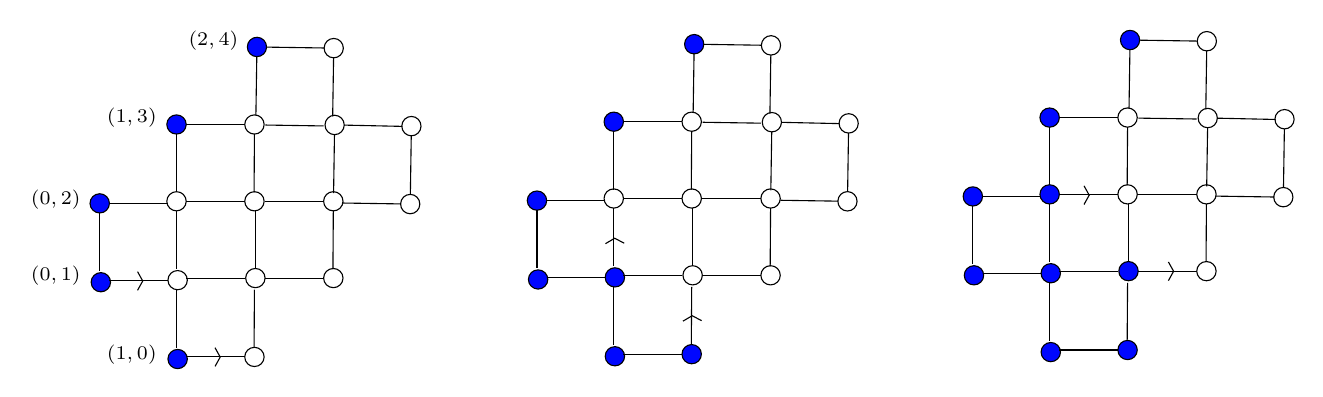
\begin{tikzpicture}[x=0.75pt,y=0.75pt,yscale=-1,xscale=1]
%uncomment if require: \path (0,3166); %set diagram left start at 0, and has height of 3166

%Shape: Ellipse [id:dp7069894143098925] 
\draw  [fill={rgb, 255:red, 0; green, 7; blue, 255 }  ,fill opacity=1 ] (92.1,67.37) .. controls (92.1,64.82) and (94.19,62.75) .. (96.77,62.75) .. controls (99.35,62.75) and (101.44,64.82) .. (101.44,67.37) .. controls (101.44,69.93) and (99.35,72) .. (96.77,72) .. controls (94.19,72) and (92.1,69.93) .. (92.1,67.37) -- cycle ;
%Shape: Ellipse [id:dp12839461897295334] 
\draw   (129.65,67.37) .. controls (129.65,64.82) and (131.74,62.75) .. (134.32,62.75) .. controls (136.9,62.75) and (138.99,64.82) .. (138.99,67.37) .. controls (138.99,69.93) and (136.9,72) .. (134.32,72) .. controls (131.74,72) and (129.65,69.93) .. (129.65,67.37) -- cycle ;
%Straight Lines [id:da35866711445955046] 
\draw    (101.44,67.37) -- (129.65,67.37) ;
%Straight Lines [id:da43190790865669115] 
\draw    (96.77,72) -- (96.77,100.04) ;
%Straight Lines [id:da9944909497211296] 
\draw    (134.32,72) -- (134.14,100.04) ;
%Shape: Ellipse [id:dp6701931517847056] 
\draw   (92.1,104.37) .. controls (92.1,101.82) and (94.19,99.75) .. (96.77,99.75) .. controls (99.35,99.75) and (101.44,101.82) .. (101.44,104.37) .. controls (101.44,106.93) and (99.35,109) .. (96.77,109) .. controls (94.19,109) and (92.1,106.93) .. (92.1,104.37) -- cycle ;
%Shape: Ellipse [id:dp010098778158842525] 
\draw   (129.65,104.37) .. controls (129.65,101.82) and (131.74,99.75) .. (134.32,99.75) .. controls (136.9,99.75) and (138.99,101.82) .. (138.99,104.37) .. controls (138.99,106.93) and (136.9,109) .. (134.32,109) .. controls (131.74,109) and (129.65,106.93) .. (129.65,104.37) -- cycle ;
%Straight Lines [id:da6322712268953989] 
\draw    (101.44,104.37) -- (129.65,104.37) ;
%Shape: Ellipse [id:dp40548932230712975] 
\draw   (167.65,104.37) .. controls (167.65,101.82) and (169.74,99.75) .. (172.32,99.75) .. controls (174.9,99.75) and (176.99,101.82) .. (176.99,104.37) .. controls (176.99,106.93) and (174.9,109) .. (172.32,109) .. controls (169.74,109) and (167.65,106.93) .. (167.65,104.37) -- cycle ;
%Straight Lines [id:da8994384711605483] 
\draw    (139.44,104.37) -- (167.65,104.37) ;
%Straight Lines [id:da11820438593814386] 
\draw    (134.77,109) -- (134.77,137.04) ;
%Straight Lines [id:da6189147012134901] 
\draw    (172.32,109) -- (172.14,137.04) ;
%Shape: Ellipse [id:dp41251727948653927] 
\draw   (130.1,141.37) .. controls (130.1,138.82) and (132.19,136.75) .. (134.77,136.75) .. controls (137.35,136.75) and (139.44,138.82) .. (139.44,141.37) .. controls (139.44,143.93) and (137.35,146) .. (134.77,146) .. controls (132.19,146) and (130.1,143.93) .. (130.1,141.37) -- cycle ;
%Shape: Ellipse [id:dp5489783626982473] 
\draw   (167.65,141.37) .. controls (167.65,138.82) and (169.74,136.75) .. (172.32,136.75) .. controls (174.9,136.75) and (176.99,138.82) .. (176.99,141.37) .. controls (176.99,143.93) and (174.9,146) .. (172.32,146) .. controls (169.74,146) and (167.65,143.93) .. (167.65,141.37) -- cycle ;
%Straight Lines [id:da8852713675152548] 
\draw    (139.44,141.37) -- (167.65,141.37) ;
%Shape: Ellipse [id:dp05976921420487358] 
\draw   (172.88,72.27) .. controls (170.32,72.24) and (168.28,70.11) .. (168.32,67.53) .. controls (168.36,64.95) and (170.47,62.9) .. (173.02,62.93) .. controls (175.58,62.97) and (177.62,65.1) .. (177.58,67.68) .. controls (177.54,70.25) and (175.43,72.31) .. (172.88,72.27) -- cycle ;
%Straight Lines [id:da5311564860786414] 
\draw    (172.45,100.48) -- (172.88,72.27) ;
%Straight Lines [id:da9685879201490818] 
\draw    (177,105.22) -- (205.04,105.65) ;
%Straight Lines [id:da8939318140306642] 
\draw    (177.58,67.68) -- (205.61,68.29) ;
%Shape: Ellipse [id:dp7953584758631467] 
\draw   (209.3,110.39) .. controls (206.74,110.35) and (204.7,108.23) .. (204.74,105.65) .. controls (204.78,103.07) and (206.89,101.01) .. (209.44,101.05) .. controls (212,101.09) and (214.04,103.21) .. (214,105.79) .. controls (213.96,108.37) and (211.85,110.43) .. (209.3,110.39) -- cycle ;
%Shape: Ellipse [id:dp3390956333842329] 
\draw   (209.87,72.84) .. controls (207.32,72.8) and (205.28,70.68) .. (205.32,68.1) .. controls (205.36,65.52) and (207.46,63.46) .. (210.02,63.5) .. controls (212.57,63.54) and (214.61,65.66) .. (214.57,68.24) .. controls (214.53,70.82) and (212.43,72.88) .. (209.87,72.84) -- cycle ;
%Straight Lines [id:da010655226579383226] 
\draw    (209.44,101.05) -- (209.87,72.84) ;
%Shape: Ellipse [id:dp9532509614740527] 
\draw  [fill={rgb, 255:red, 0; green, 7; blue, 255 }  ,fill opacity=1 ] (135.45,34.7) .. controls (132.9,34.66) and (130.86,32.53) .. (130.9,29.95) .. controls (130.94,27.37) and (133.04,25.32) .. (135.6,25.36) .. controls (138.15,25.39) and (140.19,27.52) .. (140.15,30.1) .. controls (140.11,32.68) and (138.01,34.73) .. (135.45,34.7) -- cycle ;
%Straight Lines [id:da1638144245344011] 
\draw    (135.02,62.9) -- (135.45,34.7) ;
%Straight Lines [id:da8177914388365325] 
\draw    (139.57,67.64) -- (167.61,68.08) ;
%Straight Lines [id:da21812020882281735] 
\draw    (140.15,30.1) -- (167.89,30.52) ;
%Shape: Ellipse [id:dp7725028982966824] 
\draw   (172.45,35.26) .. controls (169.89,35.22) and (167.85,33.1) .. (167.89,30.52) .. controls (167.93,27.94) and (170.04,25.88) .. (172.59,25.92) .. controls (175.15,25.96) and (177.18,28.09) .. (177.15,30.66) .. controls (177.11,33.24) and (175,35.3) .. (172.45,35.26) -- cycle ;
%Straight Lines [id:da9536661438970797] 
\draw    (172.01,63.47) -- (172.45,35.26) ;
%Shape: Ellipse [id:dp7448293525884772] 
\draw   (92.65,142.37) .. controls (92.65,139.82) and (94.74,137.75) .. (97.32,137.75) .. controls (99.9,137.75) and (101.99,139.82) .. (101.99,142.37) .. controls (101.99,144.93) and (99.9,147) .. (97.32,147) .. controls (94.74,147) and (92.65,144.93) .. (92.65,142.37) -- cycle ;
%Straight Lines [id:da3628730785197847] 
\draw    (96.77,109) -- (96.77,137.04) ;
%Straight Lines [id:da15921262236665246] 
\draw    (101.44,141.37) -- (129.65,141.37) ;
%Shape: Ellipse [id:dp39097413822139904] 
\draw  [fill={rgb, 255:red, 0; green, 7; blue, 255 }  ,fill opacity=1 ] (55.65,143.37) .. controls (55.65,140.82) and (57.74,138.75) .. (60.32,138.75) .. controls (62.9,138.75) and (64.99,140.82) .. (64.99,143.37) .. controls (64.99,145.93) and (62.9,148) .. (60.32,148) .. controls (57.74,148) and (55.65,145.93) .. (55.65,143.37) -- cycle ;
%Shape: Ellipse [id:dp08464088056579244] 
\draw  [fill={rgb, 255:red, 0; green, 7; blue, 255 }  ,fill opacity=1 ] (55.1,105.37) .. controls (55.1,102.82) and (57.19,100.75) .. (59.77,100.75) .. controls (62.35,100.75) and (64.44,102.82) .. (64.44,105.37) .. controls (64.44,107.93) and (62.35,110) .. (59.77,110) .. controls (57.19,110) and (55.1,107.93) .. (55.1,105.37) -- cycle ;
%Straight Lines [id:da48311473975397756] 
\draw    (64.44,105.37) -- (92.65,105.37) ;
%Straight Lines [id:da2546106348581565] 
\draw    (59.77,110) -- (59.77,138.04) ;
%Straight Lines [id:da6009554771575353] 
\draw    (64.44,142.37) -- (92.65,142.37) ;
%Shape: Ellipse [id:dp9727361394866706] 
\draw  [fill={rgb, 255:red, 0; green, 7; blue, 255 }  ,fill opacity=1 ] (92.65,180.37) .. controls (92.65,177.82) and (94.74,175.75) .. (97.32,175.75) .. controls (99.9,175.75) and (101.99,177.82) .. (101.99,180.37) .. controls (101.99,182.93) and (99.9,185) .. (97.32,185) .. controls (94.74,185) and (92.65,182.93) .. (92.65,180.37) -- cycle ;
%Straight Lines [id:da22653657369826685] 
\draw    (96.77,147) -- (96.77,175.04) ;
%Straight Lines [id:da7560057906284208] 
\draw    (134.32,147) -- (134.14,175.04) ;
%Shape: Ellipse [id:dp8681048023864941] 
\draw  [fill={rgb, 255:red, 255; green, 255; blue, 255 }  ,fill opacity=1 ] (129.65,179.37) .. controls (129.65,176.82) and (131.74,174.75) .. (134.32,174.75) .. controls (136.9,174.75) and (138.99,176.82) .. (138.99,179.37) .. controls (138.99,181.93) and (136.9,184) .. (134.32,184) .. controls (131.74,184) and (129.65,181.93) .. (129.65,179.37) -- cycle ;
%Straight Lines [id:da999872098402571] 
\draw    (101.44,179.37) -- (129.65,179.37) ;
%Shape: Ellipse [id:dp13624108419111147] 
\draw  [fill={rgb, 255:red, 0; green, 7; blue, 255 }  ,fill opacity=1 ] (302.77,66.04) .. controls (302.77,63.48) and (304.86,61.41) .. (307.44,61.41) .. controls (310.02,61.41) and (312.11,63.48) .. (312.11,66.04) .. controls (312.11,68.6) and (310.02,70.67) .. (307.44,70.67) .. controls (304.86,70.67) and (302.77,68.6) .. (302.77,66.04) -- cycle ;
%Shape: Ellipse [id:dp06030376906256396] 
\draw   (340.32,66.04) .. controls (340.32,63.48) and (342.41,61.41) .. (344.99,61.41) .. controls (347.57,61.41) and (349.66,63.48) .. (349.66,66.04) .. controls (349.66,68.6) and (347.57,70.67) .. (344.99,70.67) .. controls (342.41,70.67) and (340.32,68.6) .. (340.32,66.04) -- cycle ;
%Straight Lines [id:da026105836305850394] 
\draw    (312.11,66.04) -- (340.32,66.04) ;
%Straight Lines [id:da74736267619638] 
\draw    (307.44,70.67) -- (307.44,98.71) ;
%Straight Lines [id:da3723939674183755] 
\draw    (344.99,70.67) -- (344.8,98.71) ;
%Shape: Ellipse [id:dp9148721515552262] 
\draw   (302.77,103.04) .. controls (302.77,100.48) and (304.86,98.41) .. (307.44,98.41) .. controls (310.02,98.41) and (312.11,100.48) .. (312.11,103.04) .. controls (312.11,105.6) and (310.02,107.67) .. (307.44,107.67) .. controls (304.86,107.67) and (302.77,105.6) .. (302.77,103.04) -- cycle ;
%Shape: Ellipse [id:dp7452686719756115] 
\draw   (340.32,103.04) .. controls (340.32,100.48) and (342.41,98.41) .. (344.99,98.41) .. controls (347.57,98.41) and (349.66,100.48) .. (349.66,103.04) .. controls (349.66,105.6) and (347.57,107.67) .. (344.99,107.67) .. controls (342.41,107.67) and (340.32,105.6) .. (340.32,103.04) -- cycle ;
%Straight Lines [id:da18350998291211384] 
\draw    (312.11,103.04) -- (340.32,103.04) ;
%Shape: Ellipse [id:dp2513284704814871] 
\draw   (378.32,103.04) .. controls (378.32,100.48) and (380.41,98.41) .. (382.99,98.41) .. controls (385.57,98.41) and (387.66,100.48) .. (387.66,103.04) .. controls (387.66,105.6) and (385.57,107.67) .. (382.99,107.67) .. controls (380.41,107.67) and (378.32,105.6) .. (378.32,103.04) -- cycle ;
%Straight Lines [id:da32091572276680125] 
\draw    (350.11,103.04) -- (378.32,103.04) ;
%Straight Lines [id:da046351659120776434] 
\draw    (345.44,107.67) -- (345.44,135.71) ;
%Straight Lines [id:da5249338647625603] 
\draw    (382.99,107.67) -- (382.8,135.71) ;
%Shape: Ellipse [id:dp9422242716937922] 
\draw   (340.77,140.04) .. controls (340.77,137.48) and (342.86,135.41) .. (345.44,135.41) .. controls (348.02,135.41) and (350.11,137.48) .. (350.11,140.04) .. controls (350.11,142.6) and (348.02,144.67) .. (345.44,144.67) .. controls (342.86,144.67) and (340.77,142.6) .. (340.77,140.04) -- cycle ;
%Shape: Ellipse [id:dp34012148555891364] 
\draw   (378.32,140.04) .. controls (378.32,137.48) and (380.41,135.41) .. (382.99,135.41) .. controls (385.57,135.41) and (387.66,137.48) .. (387.66,140.04) .. controls (387.66,142.6) and (385.57,144.67) .. (382.99,144.67) .. controls (380.41,144.67) and (378.32,142.6) .. (378.32,140.04) -- cycle ;
%Straight Lines [id:da9859680115879758] 
\draw    (350.11,140.04) -- (378.32,140.04) ;
%Shape: Ellipse [id:dp8220327204344716] 
\draw   (383.55,70.94) .. controls (380.99,70.9) and (378.95,68.78) .. (378.99,66.2) .. controls (379.03,63.62) and (381.13,61.56) .. (383.69,61.6) .. controls (386.24,61.64) and (388.28,63.76) .. (388.24,66.34) .. controls (388.2,68.92) and (386.1,70.98) .. (383.55,70.94) -- cycle ;
%Straight Lines [id:da9714606623566501] 
\draw    (383.11,99.15) -- (383.55,70.94) ;
%Straight Lines [id:da044712843530642976] 
\draw    (387.67,103.89) -- (415.7,104.32) ;
%Straight Lines [id:da6246800419365646] 
\draw    (388.24,66.34) -- (416.28,66.96) ;
%Shape: Ellipse [id:dp01628649823302164] 
\draw   (419.96,109.06) .. controls (417.41,109.02) and (415.37,106.9) .. (415.41,104.32) .. controls (415.45,101.74) and (417.55,99.68) .. (420.11,99.72) .. controls (422.66,99.76) and (424.7,101.88) .. (424.66,104.46) .. controls (424.62,107.04) and (422.52,109.1) .. (419.96,109.06) -- cycle ;
%Shape: Ellipse [id:dp37229383958358575] 
\draw   (420.54,71.51) .. controls (417.99,71.47) and (415.95,69.35) .. (415.99,66.77) .. controls (416.03,64.19) and (418.13,62.13) .. (420.68,62.17) .. controls (423.24,62.21) and (425.28,64.33) .. (425.24,66.91) .. controls (425.2,69.49) and (423.1,71.55) .. (420.54,71.51) -- cycle ;
%Straight Lines [id:da31063965597405196] 
\draw    (420.11,99.72) -- (420.54,71.51) ;
%Shape: Ellipse [id:dp8103069506580036] 
\draw  [fill={rgb, 255:red, 0; green, 7; blue, 255 }  ,fill opacity=1 ] (346.12,33.36) .. controls (343.56,33.32) and (341.52,31.2) .. (341.56,28.62) .. controls (341.6,26.04) and (343.71,23.98) .. (346.26,24.02) .. controls (348.82,24.06) and (350.86,26.18) .. (350.82,28.76) .. controls (350.78,31.34) and (348.67,33.4) .. (346.12,33.36) -- cycle ;
%Straight Lines [id:da16573297041554758] 
\draw    (345.69,61.57) -- (346.12,33.36) ;
%Straight Lines [id:da2736516376753677] 
\draw    (350.24,66.31) -- (378.27,66.74) ;
%Straight Lines [id:da535500643101059] 
\draw    (350.82,28.76) -- (378.56,29.19) ;
%Shape: Ellipse [id:dp0834863586494361] 
\draw   (383.11,33.93) .. controls (380.56,33.89) and (378.52,31.77) .. (378.56,29.19) .. controls (378.6,26.61) and (380.7,24.55) .. (383.26,24.59) .. controls (385.81,24.63) and (387.85,26.75) .. (387.81,29.33) .. controls (387.77,31.91) and (385.67,33.97) .. (383.11,33.93) -- cycle ;
%Straight Lines [id:da5555898440914054] 
\draw    (382.68,62.14) -- (383.11,33.93) ;
%Shape: Ellipse [id:dp9874545463855635] 
\draw  [fill={rgb, 255:red, 0; green, 7; blue, 255 }  ,fill opacity=1 ] (303.32,141.04) .. controls (303.32,138.48) and (305.41,136.41) .. (307.99,136.41) .. controls (310.57,136.41) and (312.66,138.48) .. (312.66,141.04) .. controls (312.66,143.6) and (310.57,145.67) .. (307.99,145.67) .. controls (305.41,145.67) and (303.32,143.6) .. (303.32,141.04) -- cycle ;
%Straight Lines [id:da0061021300085255525] 
\draw    (307.44,107.67) -- (307.44,135.71) ;
%Straight Lines [id:da1279364277428876] 
\draw    (312.11,140.04) -- (340.32,140.04) ;
%Shape: Ellipse [id:dp49263457258055143] 
\draw  [fill={rgb, 255:red, 0; green, 7; blue, 255 }  ,fill opacity=1 ] (266.32,142.04) .. controls (266.32,139.48) and (268.41,137.41) .. (270.99,137.41) .. controls (273.57,137.41) and (275.66,139.48) .. (275.66,142.04) .. controls (275.66,144.6) and (273.57,146.67) .. (270.99,146.67) .. controls (268.41,146.67) and (266.32,144.6) .. (266.32,142.04) -- cycle ;
%Shape: Ellipse [id:dp3341112585359639] 
\draw  [fill={rgb, 255:red, 0; green, 7; blue, 255 }  ,fill opacity=1 ] (265.77,104.04) .. controls (265.77,101.48) and (267.86,99.41) .. (270.44,99.41) .. controls (273.02,99.41) and (275.11,101.48) .. (275.11,104.04) .. controls (275.11,106.6) and (273.02,108.67) .. (270.44,108.67) .. controls (267.86,108.67) and (265.77,106.6) .. (265.77,104.04) -- cycle ;
%Straight Lines [id:da28287677990600046] 
\draw    (275.11,104.04) -- (303.32,104.04) ;
%Straight Lines [id:da3266397650724694] 
\draw    (270.44,108.67) -- (270.44,136.71) ;
%Straight Lines [id:da2713487154539739] 
\draw    (275.11,141.04) -- (303.32,141.04) ;
%Shape: Ellipse [id:dp6474304142710697] 
\draw  [fill={rgb, 255:red, 0; green, 7; blue, 255 }  ,fill opacity=1 ] (303.32,179.04) .. controls (303.32,176.48) and (305.41,174.41) .. (307.99,174.41) .. controls (310.57,174.41) and (312.66,176.48) .. (312.66,179.04) .. controls (312.66,181.6) and (310.57,183.67) .. (307.99,183.67) .. controls (305.41,183.67) and (303.32,181.6) .. (303.32,179.04) -- cycle ;
%Straight Lines [id:da3793384302346873] 
\draw    (307.44,145.67) -- (307.44,173.71) ;
%Straight Lines [id:da3041491833421809] 
\draw    (344.99,145.67) -- (344.8,173.71) ;
%Shape: Ellipse [id:dp17970199633866601] 
\draw  [fill={rgb, 255:red, 0; green, 7; blue, 255 }  ,fill opacity=1 ] (340.32,178.04) .. controls (340.32,175.48) and (342.41,173.41) .. (344.99,173.41) .. controls (347.57,173.41) and (349.66,175.48) .. (349.66,178.04) .. controls (349.66,180.6) and (347.57,182.67) .. (344.99,182.67) .. controls (342.41,182.67) and (340.32,180.6) .. (340.32,178.04) -- cycle ;
%Straight Lines [id:da019918135066070097] 
\draw    (312.11,178.04) -- (340.32,178.04) ;
\draw   (115.33,174.93) -- (117.83,179.43) -- (115.33,183.93) ;
\draw   (78,138.27) -- (80.5,142.77) -- (78,147.27) ;
%Shape: Ellipse [id:dp003891085355659629] 
\draw  [fill={rgb, 255:red, 0; green, 7; blue, 255 }  ,fill opacity=1 ] (512.77,64.04) .. controls (512.77,61.48) and (514.86,59.41) .. (517.44,59.41) .. controls (520.02,59.41) and (522.11,61.48) .. (522.11,64.04) .. controls (522.11,66.6) and (520.02,68.67) .. (517.44,68.67) .. controls (514.86,68.67) and (512.77,66.6) .. (512.77,64.04) -- cycle ;
%Shape: Ellipse [id:dp337682257162918] 
\draw   (550.32,64.04) .. controls (550.32,61.48) and (552.41,59.41) .. (554.99,59.41) .. controls (557.57,59.41) and (559.66,61.48) .. (559.66,64.04) .. controls (559.66,66.6) and (557.57,68.67) .. (554.99,68.67) .. controls (552.41,68.67) and (550.32,66.6) .. (550.32,64.04) -- cycle ;
%Straight Lines [id:da3721572367239261] 
\draw    (522.11,64.04) -- (550.32,64.04) ;
%Straight Lines [id:da6034157827268747] 
\draw    (517.44,68.67) -- (517.44,96.71) ;
%Straight Lines [id:da6581299440250502] 
\draw    (554.99,68.67) -- (554.8,96.71) ;
%Shape: Ellipse [id:dp5805462331897108] 
\draw  [fill={rgb, 255:red, 0; green, 7; blue, 255 }  ,fill opacity=1 ] (512.77,101.04) .. controls (512.77,98.48) and (514.86,96.41) .. (517.44,96.41) .. controls (520.02,96.41) and (522.11,98.48) .. (522.11,101.04) .. controls (522.11,103.6) and (520.02,105.67) .. (517.44,105.67) .. controls (514.86,105.67) and (512.77,103.6) .. (512.77,101.04) -- cycle ;
%Shape: Ellipse [id:dp31322454364826136] 
\draw   (550.32,101.04) .. controls (550.32,98.48) and (552.41,96.41) .. (554.99,96.41) .. controls (557.57,96.41) and (559.66,98.48) .. (559.66,101.04) .. controls (559.66,103.6) and (557.57,105.67) .. (554.99,105.67) .. controls (552.41,105.67) and (550.32,103.6) .. (550.32,101.04) -- cycle ;
%Straight Lines [id:da46623484932817505] 
\draw    (522.11,101.04) -- (550.32,101.04) ;
%Shape: Ellipse [id:dp5279901342416101] 
\draw   (588.32,101.04) .. controls (588.32,98.48) and (590.41,96.41) .. (592.99,96.41) .. controls (595.57,96.41) and (597.66,98.48) .. (597.66,101.04) .. controls (597.66,103.6) and (595.57,105.67) .. (592.99,105.67) .. controls (590.41,105.67) and (588.32,103.6) .. (588.32,101.04) -- cycle ;
%Straight Lines [id:da45028754730739884] 
\draw    (560.11,101.04) -- (588.32,101.04) ;
%Straight Lines [id:da6524747502332668] 
\draw    (555.44,105.67) -- (555.44,133.71) ;
%Straight Lines [id:da9846251994333522] 
\draw    (592.99,105.67) -- (592.8,133.71) ;
%Shape: Ellipse [id:dp23833950421355776] 
\draw  [fill={rgb, 255:red, 0; green, 7; blue, 255 }  ,fill opacity=1 ] (550.77,138.04) .. controls (550.77,135.48) and (552.86,133.41) .. (555.44,133.41) .. controls (558.02,133.41) and (560.11,135.48) .. (560.11,138.04) .. controls (560.11,140.6) and (558.02,142.67) .. (555.44,142.67) .. controls (552.86,142.67) and (550.77,140.6) .. (550.77,138.04) -- cycle ;
%Shape: Ellipse [id:dp835345217577697] 
\draw   (588.32,138.04) .. controls (588.32,135.48) and (590.41,133.41) .. (592.99,133.41) .. controls (595.57,133.41) and (597.66,135.48) .. (597.66,138.04) .. controls (597.66,140.6) and (595.57,142.67) .. (592.99,142.67) .. controls (590.41,142.67) and (588.32,140.6) .. (588.32,138.04) -- cycle ;
%Straight Lines [id:da24086001925750755] 
\draw    (560.11,138.04) -- (588.32,138.04) ;
%Shape: Ellipse [id:dp3202335051789542] 
\draw   (593.55,68.94) .. controls (590.99,68.9) and (588.95,66.78) .. (588.99,64.2) .. controls (589.03,61.62) and (591.13,59.56) .. (593.69,59.6) .. controls (596.24,59.64) and (598.28,61.76) .. (598.24,64.34) .. controls (598.2,66.92) and (596.1,68.98) .. (593.55,68.94) -- cycle ;
%Straight Lines [id:da6053801262963364] 
\draw    (593.11,97.15) -- (593.55,68.94) ;
%Straight Lines [id:da0749727586573331] 
\draw    (597.67,101.89) -- (625.7,102.32) ;
%Straight Lines [id:da3746005855341382] 
\draw    (598.24,64.34) -- (626.28,64.96) ;
%Shape: Ellipse [id:dp14763783088013105] 
\draw   (629.96,107.06) .. controls (627.41,107.02) and (625.37,104.9) .. (625.41,102.32) .. controls (625.45,99.74) and (627.55,97.68) .. (630.11,97.72) .. controls (632.66,97.76) and (634.7,99.88) .. (634.66,102.46) .. controls (634.62,105.04) and (632.52,107.1) .. (629.96,107.06) -- cycle ;
%Shape: Ellipse [id:dp6885692966994197] 
\draw   (630.54,69.51) .. controls (627.99,69.47) and (625.95,67.35) .. (625.99,64.77) .. controls (626.03,62.19) and (628.13,60.13) .. (630.68,60.17) .. controls (633.24,60.21) and (635.28,62.33) .. (635.24,64.91) .. controls (635.2,67.49) and (633.1,69.55) .. (630.54,69.51) -- cycle ;
%Straight Lines [id:da5274842321057884] 
\draw    (630.11,97.72) -- (630.54,69.51) ;
%Shape: Ellipse [id:dp8691169349984225] 
\draw  [fill={rgb, 255:red, 0; green, 7; blue, 255 }  ,fill opacity=1 ] (556.12,31.36) .. controls (553.56,31.32) and (551.52,29.2) .. (551.56,26.62) .. controls (551.6,24.04) and (553.71,21.98) .. (556.26,22.02) .. controls (558.82,22.06) and (560.86,24.18) .. (560.82,26.76) .. controls (560.78,29.34) and (558.67,31.4) .. (556.12,31.36) -- cycle ;
%Straight Lines [id:da24826602746958193] 
\draw    (555.69,59.57) -- (556.12,31.36) ;
%Straight Lines [id:da21199546592236407] 
\draw    (560.24,64.31) -- (588.27,64.74) ;
%Straight Lines [id:da029348569198964225] 
\draw    (560.82,26.76) -- (588.56,27.19) ;
%Shape: Ellipse [id:dp707973471893413] 
\draw   (593.11,31.93) .. controls (590.56,31.89) and (588.52,29.77) .. (588.56,27.19) .. controls (588.6,24.61) and (590.7,22.55) .. (593.26,22.59) .. controls (595.81,22.63) and (597.85,24.75) .. (597.81,27.33) .. controls (597.77,29.91) and (595.67,31.97) .. (593.11,31.93) -- cycle ;
%Straight Lines [id:da4408385413696264] 
\draw    (592.68,60.14) -- (593.11,31.93) ;
%Shape: Ellipse [id:dp6824542286754107] 
\draw  [fill={rgb, 255:red, 0; green, 7; blue, 255 }  ,fill opacity=1 ] (513.32,139.04) .. controls (513.32,136.48) and (515.41,134.41) .. (517.99,134.41) .. controls (520.57,134.41) and (522.66,136.48) .. (522.66,139.04) .. controls (522.66,141.6) and (520.57,143.67) .. (517.99,143.67) .. controls (515.41,143.67) and (513.32,141.6) .. (513.32,139.04) -- cycle ;
%Straight Lines [id:da8965189993652262] 
\draw    (517.44,105.67) -- (517.44,133.71) ;
%Straight Lines [id:da22295218728252675] 
\draw    (522.11,138.04) -- (550.32,138.04) ;
%Shape: Ellipse [id:dp871052871656841] 
\draw  [fill={rgb, 255:red, 0; green, 7; blue, 255 }  ,fill opacity=1 ] (476.32,140.04) .. controls (476.32,137.48) and (478.41,135.41) .. (480.99,135.41) .. controls (483.57,135.41) and (485.66,137.48) .. (485.66,140.04) .. controls (485.66,142.6) and (483.57,144.67) .. (480.99,144.67) .. controls (478.41,144.67) and (476.32,142.6) .. (476.32,140.04) -- cycle ;
%Shape: Ellipse [id:dp14561512001916732] 
\draw  [fill={rgb, 255:red, 0; green, 7; blue, 255 }  ,fill opacity=1 ] (475.77,102.04) .. controls (475.77,99.48) and (477.86,97.41) .. (480.44,97.41) .. controls (483.02,97.41) and (485.11,99.48) .. (485.11,102.04) .. controls (485.11,104.6) and (483.02,106.67) .. (480.44,106.67) .. controls (477.86,106.67) and (475.77,104.6) .. (475.77,102.04) -- cycle ;
%Straight Lines [id:da7105903182068207] 
\draw    (485.11,102.04) -- (513.32,102.04) ;
%Straight Lines [id:da40043238176958673] 
\draw    (480.44,106.67) -- (480.44,134.71) ;
%Straight Lines [id:da05884657615886568] 
\draw    (485.11,139.04) -- (513.32,139.04) ;
%Shape: Ellipse [id:dp6943042013383234] 
\draw  [fill={rgb, 255:red, 0; green, 7; blue, 255 }  ,fill opacity=1 ] (513.32,177.04) .. controls (513.32,174.48) and (515.41,172.41) .. (517.99,172.41) .. controls (520.57,172.41) and (522.66,174.48) .. (522.66,177.04) .. controls (522.66,179.6) and (520.57,181.67) .. (517.99,181.67) .. controls (515.41,181.67) and (513.32,179.6) .. (513.32,177.04) -- cycle ;
%Straight Lines [id:da8808919853545881] 
\draw    (517.44,143.67) -- (517.44,171.71) ;
%Straight Lines [id:da10003754217827565] 
\draw    (554.99,143.67) -- (554.8,171.71) ;
%Shape: Ellipse [id:dp5420061485885599] 
\draw  [fill={rgb, 255:red, 0; green, 7; blue, 255 }  ,fill opacity=1 ] (550.32,176.04) .. controls (550.32,173.48) and (552.41,171.41) .. (554.99,171.41) .. controls (557.57,171.41) and (559.66,173.48) .. (559.66,176.04) .. controls (559.66,178.6) and (557.57,180.67) .. (554.99,180.67) .. controls (552.41,180.67) and (550.32,178.6) .. (550.32,176.04) -- cycle ;
%Straight Lines [id:da13889454187544714] 
\draw    (522.11,176.04) -- (550.32,176.04) ;
\draw   (303.45,124.8) -- (307.89,122.18) -- (312.45,124.57) ;
\draw   (340.78,162.13) -- (345.22,159.52) -- (349.78,161.9) ;
\draw   (534,96.93) -- (536.5,101.43) -- (534,105.93) ;
\draw   (574.67,133.6) -- (577.17,138.1) -- (574.67,142.6) ;

% Text Node
\draw (62,172.33) node [anchor=north west][inner sep=0.75pt]  [font=\scriptsize]  {$( 1,0)$};
% Text Node
\draw (25.33,134.33) node [anchor=north west][inner sep=0.75pt]  [font=\scriptsize]  {$( 0,1)$};
% Text Node
\draw (25.33,97.67) node [anchor=north west][inner sep=0.75pt]  [font=\scriptsize]  {$( 0,2)$};
% Text Node
\draw (62,58.33) node [anchor=north west][inner sep=0.75pt]  [font=\scriptsize]  {$( 1,3)$};
% Text Node
\draw (101.33,21) node [anchor=north west][inner sep=0.75pt]  [font=\scriptsize]  {$( 2,4)$};


\end{tikzpicture}
    \caption{Ordering of forces given by forcing process $F_2$}
    \label{fig:F2Process}
\end{figure}

\begin{figure}[h!]
    \centering



\tikzset{every picture/.style={line width=0.75pt}} %set default line width to 0.75pt        

       

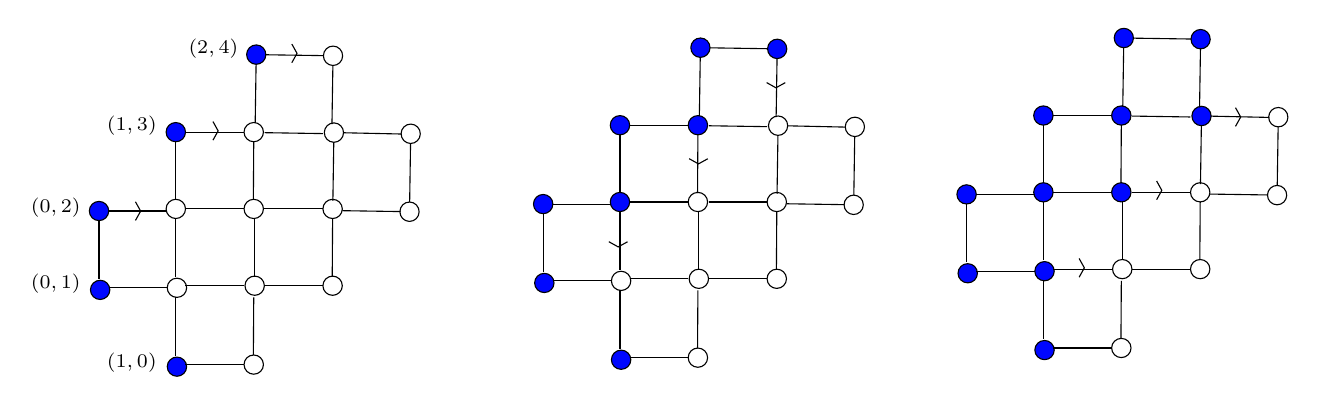
\begin{tikzpicture}[x=0.75pt,y=0.75pt,yscale=-1,xscale=1]
%uncomment if require: \path (0,3166); %set diagram left start at 0, and has height of 3166

%Shape: Ellipse [id:dp6930170898661223] 
\draw  [fill={rgb, 255:red, 0; green, 7; blue, 255 }  ,fill opacity=1 ] (90.1,275.37) .. controls (90.1,272.82) and (92.19,270.75) .. (94.77,270.75) .. controls (97.35,270.75) and (99.44,272.82) .. (99.44,275.37) .. controls (99.44,277.93) and (97.35,280) .. (94.77,280) .. controls (92.19,280) and (90.1,277.93) .. (90.1,275.37) -- cycle ;
%Shape: Ellipse [id:dp5784322848270685] 
\draw   (127.65,275.37) .. controls (127.65,272.82) and (129.74,270.75) .. (132.32,270.75) .. controls (134.9,270.75) and (136.99,272.82) .. (136.99,275.37) .. controls (136.99,277.93) and (134.9,280) .. (132.32,280) .. controls (129.74,280) and (127.65,277.93) .. (127.65,275.37) -- cycle ;
%Straight Lines [id:da7447088143352298] 
\draw    (99.44,275.37) -- (127.65,275.37) ;
%Straight Lines [id:da27024055730741736] 
\draw    (94.77,280) -- (94.77,308.04) ;
%Straight Lines [id:da07620427442556543] 
\draw    (132.32,280) -- (132.14,308.04) ;
%Shape: Ellipse [id:dp5849256087081274] 
\draw   (90.1,312.37) .. controls (90.1,309.82) and (92.19,307.75) .. (94.77,307.75) .. controls (97.35,307.75) and (99.44,309.82) .. (99.44,312.37) .. controls (99.44,314.93) and (97.35,317) .. (94.77,317) .. controls (92.19,317) and (90.1,314.93) .. (90.1,312.37) -- cycle ;
%Shape: Ellipse [id:dp7303679971641182] 
\draw   (127.65,312.37) .. controls (127.65,309.82) and (129.74,307.75) .. (132.32,307.75) .. controls (134.9,307.75) and (136.99,309.82) .. (136.99,312.37) .. controls (136.99,314.93) and (134.9,317) .. (132.32,317) .. controls (129.74,317) and (127.65,314.93) .. (127.65,312.37) -- cycle ;
%Straight Lines [id:da5855356003680329] 
\draw    (99.44,312.37) -- (127.65,312.37) ;
%Shape: Ellipse [id:dp9061240003849841] 
\draw   (165.65,312.37) .. controls (165.65,309.82) and (167.74,307.75) .. (170.32,307.75) .. controls (172.9,307.75) and (174.99,309.82) .. (174.99,312.37) .. controls (174.99,314.93) and (172.9,317) .. (170.32,317) .. controls (167.74,317) and (165.65,314.93) .. (165.65,312.37) -- cycle ;
%Straight Lines [id:da9490202458466189] 
\draw    (137.44,312.37) -- (165.65,312.37) ;
%Straight Lines [id:da9372622172156959] 
\draw    (132.77,317) -- (132.77,345.04) ;
%Straight Lines [id:da5770043616160666] 
\draw    (170.32,317) -- (170.14,345.04) ;
%Shape: Ellipse [id:dp5522376738897752] 
\draw   (128.1,349.37) .. controls (128.1,346.82) and (130.19,344.75) .. (132.77,344.75) .. controls (135.35,344.75) and (137.44,346.82) .. (137.44,349.37) .. controls (137.44,351.93) and (135.35,354) .. (132.77,354) .. controls (130.19,354) and (128.1,351.93) .. (128.1,349.37) -- cycle ;
%Shape: Ellipse [id:dp25429602057168266] 
\draw   (165.65,349.37) .. controls (165.65,346.82) and (167.74,344.75) .. (170.32,344.75) .. controls (172.9,344.75) and (174.99,346.82) .. (174.99,349.37) .. controls (174.99,351.93) and (172.9,354) .. (170.32,354) .. controls (167.74,354) and (165.65,351.93) .. (165.65,349.37) -- cycle ;
%Straight Lines [id:da7177032842133577] 
\draw    (137.44,349.37) -- (165.65,349.37) ;
%Shape: Ellipse [id:dp8355591183733335] 
\draw   (170.88,280.27) .. controls (168.32,280.24) and (166.28,278.11) .. (166.32,275.53) .. controls (166.36,272.95) and (168.47,270.9) .. (171.02,270.93) .. controls (173.58,270.97) and (175.62,273.1) .. (175.58,275.68) .. controls (175.54,278.25) and (173.43,280.31) .. (170.88,280.27) -- cycle ;
%Straight Lines [id:da6357503366679073] 
\draw    (170.45,308.48) -- (170.88,280.27) ;
%Straight Lines [id:da10070962974886588] 
\draw    (175,313.22) -- (203.04,313.65) ;
%Straight Lines [id:da6302823167430576] 
\draw    (175.58,275.68) -- (203.61,276.29) ;
%Shape: Ellipse [id:dp6969987857858848] 
\draw   (207.3,318.39) .. controls (204.74,318.35) and (202.7,316.23) .. (202.74,313.65) .. controls (202.78,311.07) and (204.89,309.01) .. (207.44,309.05) .. controls (210,309.09) and (212.04,311.21) .. (212,313.79) .. controls (211.96,316.37) and (209.85,318.43) .. (207.3,318.39) -- cycle ;
%Shape: Ellipse [id:dp40632945382290464] 
\draw   (207.87,280.84) .. controls (205.32,280.8) and (203.28,278.68) .. (203.32,276.1) .. controls (203.36,273.52) and (205.46,271.46) .. (208.02,271.5) .. controls (210.57,271.54) and (212.61,273.66) .. (212.57,276.24) .. controls (212.53,278.82) and (210.43,280.88) .. (207.87,280.84) -- cycle ;
%Straight Lines [id:da9099743838126804] 
\draw    (207.44,309.05) -- (207.87,280.84) ;
%Shape: Ellipse [id:dp0020596005321376065] 
\draw  [fill={rgb, 255:red, 0; green, 7; blue, 255 }  ,fill opacity=1 ] (133.45,242.7) .. controls (130.9,242.66) and (128.86,240.53) .. (128.9,237.95) .. controls (128.94,235.37) and (131.04,233.32) .. (133.6,233.36) .. controls (136.15,233.39) and (138.19,235.52) .. (138.15,238.1) .. controls (138.11,240.68) and (136.01,242.73) .. (133.45,242.7) -- cycle ;
%Straight Lines [id:da5146408147296431] 
\draw    (133.02,270.9) -- (133.45,242.7) ;
%Straight Lines [id:da6872702293610733] 
\draw    (137.57,275.64) -- (165.61,276.08) ;
%Straight Lines [id:da40582876700061443] 
\draw    (138.15,238.1) -- (165.89,238.52) ;
%Shape: Ellipse [id:dp010152427285827215] 
\draw   (170.45,243.26) .. controls (167.89,243.22) and (165.85,241.1) .. (165.89,238.52) .. controls (165.93,235.94) and (168.04,233.88) .. (170.59,233.92) .. controls (173.15,233.96) and (175.18,236.09) .. (175.15,238.66) .. controls (175.11,241.24) and (173,243.3) .. (170.45,243.26) -- cycle ;
%Straight Lines [id:da9274754783081428] 
\draw    (170.01,271.47) -- (170.45,243.26) ;
%Shape: Ellipse [id:dp588965492787938] 
\draw   (90.65,350.37) .. controls (90.65,347.82) and (92.74,345.75) .. (95.32,345.75) .. controls (97.9,345.75) and (99.99,347.82) .. (99.99,350.37) .. controls (99.99,352.93) and (97.9,355) .. (95.32,355) .. controls (92.74,355) and (90.65,352.93) .. (90.65,350.37) -- cycle ;
%Straight Lines [id:da7806802895812577] 
\draw    (94.77,317) -- (94.77,345.04) ;
%Straight Lines [id:da5185494489899437] 
\draw    (99.44,349.37) -- (127.65,349.37) ;
%Shape: Ellipse [id:dp9454232758436534] 
\draw  [fill={rgb, 255:red, 0; green, 7; blue, 255 }  ,fill opacity=1 ] (53.65,351.37) .. controls (53.65,348.82) and (55.74,346.75) .. (58.32,346.75) .. controls (60.9,346.75) and (62.99,348.82) .. (62.99,351.37) .. controls (62.99,353.93) and (60.9,356) .. (58.32,356) .. controls (55.74,356) and (53.65,353.93) .. (53.65,351.37) -- cycle ;
%Shape: Ellipse [id:dp7638811155162227] 
\draw  [fill={rgb, 255:red, 0; green, 7; blue, 255 }  ,fill opacity=1 ] (53.1,313.37) .. controls (53.1,310.82) and (55.19,308.75) .. (57.77,308.75) .. controls (60.35,308.75) and (62.44,310.82) .. (62.44,313.37) .. controls (62.44,315.93) and (60.35,318) .. (57.77,318) .. controls (55.19,318) and (53.1,315.93) .. (53.1,313.37) -- cycle ;
%Straight Lines [id:da8506205086512887] 
\draw    (62.44,313.37) -- (90.65,313.37) ;
%Straight Lines [id:da2871115942559249] 
\draw    (57.77,318) -- (57.77,346.04) ;
%Straight Lines [id:da8378160780284208] 
\draw    (62.44,350.37) -- (90.65,350.37) ;
%Shape: Ellipse [id:dp4726896999796143] 
\draw  [fill={rgb, 255:red, 0; green, 7; blue, 255 }  ,fill opacity=1 ] (90.65,388.37) .. controls (90.65,385.82) and (92.74,383.75) .. (95.32,383.75) .. controls (97.9,383.75) and (99.99,385.82) .. (99.99,388.37) .. controls (99.99,390.93) and (97.9,393) .. (95.32,393) .. controls (92.74,393) and (90.65,390.93) .. (90.65,388.37) -- cycle ;
%Straight Lines [id:da9157134899825864] 
\draw    (94.77,355) -- (94.77,383.04) ;
%Straight Lines [id:da4977877603518014] 
\draw    (132.32,355) -- (132.14,383.04) ;
%Shape: Ellipse [id:dp613419791655843] 
\draw  [fill={rgb, 255:red, 255; green, 255; blue, 255 }  ,fill opacity=1 ] (127.65,387.37) .. controls (127.65,384.82) and (129.74,382.75) .. (132.32,382.75) .. controls (134.9,382.75) and (136.99,384.82) .. (136.99,387.37) .. controls (136.99,389.93) and (134.9,392) .. (132.32,392) .. controls (129.74,392) and (127.65,389.93) .. (127.65,387.37) -- cycle ;
%Straight Lines [id:da018184614660688436] 
\draw    (99.44,387.37) -- (127.65,387.37) ;
%Shape: Ellipse [id:dp15525018793065193] 
\draw  [fill={rgb, 255:red, 0; green, 7; blue, 255 }  ,fill opacity=1 ] (304.1,272.04) .. controls (304.1,269.48) and (306.19,267.41) .. (308.77,267.41) .. controls (311.35,267.41) and (313.44,269.48) .. (313.44,272.04) .. controls (313.44,274.6) and (311.35,276.67) .. (308.77,276.67) .. controls (306.19,276.67) and (304.1,274.6) .. (304.1,272.04) -- cycle ;
%Shape: Ellipse [id:dp5274578119474227] 
\draw  [fill={rgb, 255:red, 0; green, 7; blue, 255 }  ,fill opacity=1 ] (341.65,272.04) .. controls (341.65,269.48) and (343.74,267.41) .. (346.32,267.41) .. controls (348.9,267.41) and (350.99,269.48) .. (350.99,272.04) .. controls (350.99,274.6) and (348.9,276.67) .. (346.32,276.67) .. controls (343.74,276.67) and (341.65,274.6) .. (341.65,272.04) -- cycle ;
%Straight Lines [id:da18287998728913613] 
\draw    (313.44,272.04) -- (341.65,272.04) ;
%Straight Lines [id:da4600455830980146] 
\draw    (308.77,276.67) -- (308.77,304.71) ;
%Straight Lines [id:da32863490908932436] 
\draw    (346.32,276.67) -- (346.14,304.71) ;
%Shape: Ellipse [id:dp34664212917386017] 
\draw  [fill={rgb, 255:red, 0; green, 7; blue, 255 }  ,fill opacity=1 ] (304.1,309.04) .. controls (304.1,306.48) and (306.19,304.41) .. (308.77,304.41) .. controls (311.35,304.41) and (313.44,306.48) .. (313.44,309.04) .. controls (313.44,311.6) and (311.35,313.67) .. (308.77,313.67) .. controls (306.19,313.67) and (304.1,311.6) .. (304.1,309.04) -- cycle ;
%Shape: Ellipse [id:dp6394731083766495] 
\draw   (341.65,309.04) .. controls (341.65,306.48) and (343.74,304.41) .. (346.32,304.41) .. controls (348.9,304.41) and (350.99,306.48) .. (350.99,309.04) .. controls (350.99,311.6) and (348.9,313.67) .. (346.32,313.67) .. controls (343.74,313.67) and (341.65,311.6) .. (341.65,309.04) -- cycle ;
%Straight Lines [id:da882952276424897] 
\draw    (313.44,309.04) -- (341.65,309.04) ;
%Shape: Ellipse [id:dp0013380653247087038] 
\draw   (379.65,309.04) .. controls (379.65,306.48) and (381.74,304.41) .. (384.32,304.41) .. controls (386.9,304.41) and (388.99,306.48) .. (388.99,309.04) .. controls (388.99,311.6) and (386.9,313.67) .. (384.32,313.67) .. controls (381.74,313.67) and (379.65,311.6) .. (379.65,309.04) -- cycle ;
%Straight Lines [id:da5878737268868326] 
\draw    (351.44,309.04) -- (379.65,309.04) ;
%Straight Lines [id:da7407965979405202] 
\draw    (346.77,313.67) -- (346.77,341.71) ;
%Straight Lines [id:da9055382893293176] 
\draw    (384.32,313.67) -- (384.14,341.71) ;
%Shape: Ellipse [id:dp7911406862962946] 
\draw   (342.1,346.04) .. controls (342.1,343.48) and (344.19,341.41) .. (346.77,341.41) .. controls (349.35,341.41) and (351.44,343.48) .. (351.44,346.04) .. controls (351.44,348.6) and (349.35,350.67) .. (346.77,350.67) .. controls (344.19,350.67) and (342.1,348.6) .. (342.1,346.04) -- cycle ;
%Shape: Ellipse [id:dp7798783898304442] 
\draw   (379.65,346.04) .. controls (379.65,343.48) and (381.74,341.41) .. (384.32,341.41) .. controls (386.9,341.41) and (388.99,343.48) .. (388.99,346.04) .. controls (388.99,348.6) and (386.9,350.67) .. (384.32,350.67) .. controls (381.74,350.67) and (379.65,348.6) .. (379.65,346.04) -- cycle ;
%Straight Lines [id:da6389735243504246] 
\draw    (351.44,346.04) -- (379.65,346.04) ;
%Shape: Ellipse [id:dp7729683905566632] 
\draw   (384.88,276.94) .. controls (382.32,276.9) and (380.28,274.78) .. (380.32,272.2) .. controls (380.36,269.62) and (382.47,267.56) .. (385.02,267.6) .. controls (387.58,267.64) and (389.62,269.76) .. (389.58,272.34) .. controls (389.54,274.92) and (387.43,276.98) .. (384.88,276.94) -- cycle ;
%Straight Lines [id:da4635988435293623] 
\draw    (384.45,305.15) -- (384.88,276.94) ;
%Straight Lines [id:da03633599003979571] 
\draw    (389,309.89) -- (417.04,310.32) ;
%Straight Lines [id:da5433150636657921] 
\draw    (389.58,272.34) -- (417.61,272.96) ;
%Shape: Ellipse [id:dp8816128641258256] 
\draw   (421.3,315.06) .. controls (418.74,315.02) and (416.7,312.9) .. (416.74,310.32) .. controls (416.78,307.74) and (418.89,305.68) .. (421.44,305.72) .. controls (424,305.76) and (426.04,307.88) .. (426,310.46) .. controls (425.96,313.04) and (423.85,315.1) .. (421.3,315.06) -- cycle ;
%Shape: Ellipse [id:dp2946317955262835] 
\draw   (421.87,277.51) .. controls (419.32,277.47) and (417.28,275.35) .. (417.32,272.77) .. controls (417.36,270.19) and (419.46,268.13) .. (422.02,268.17) .. controls (424.57,268.21) and (426.61,270.33) .. (426.57,272.91) .. controls (426.53,275.49) and (424.43,277.55) .. (421.87,277.51) -- cycle ;
%Straight Lines [id:da1202924130141344] 
\draw    (421.44,305.72) -- (421.87,277.51) ;
%Shape: Ellipse [id:dp6909132758112801] 
\draw  [fill={rgb, 255:red, 0; green, 7; blue, 255 }  ,fill opacity=1 ] (347.45,239.36) .. controls (344.9,239.32) and (342.86,237.2) .. (342.9,234.62) .. controls (342.94,232.04) and (345.04,229.98) .. (347.6,230.02) .. controls (350.15,230.06) and (352.19,232.18) .. (352.15,234.76) .. controls (352.11,237.34) and (350.01,239.4) .. (347.45,239.36) -- cycle ;
%Straight Lines [id:da5475934725733361] 
\draw    (347.02,267.57) -- (347.45,239.36) ;
%Straight Lines [id:da38529918718802847] 
\draw    (351.57,272.31) -- (379.61,272.74) ;
%Straight Lines [id:da5793263174028676] 
\draw    (352.15,234.76) -- (379.89,235.19) ;
%Shape: Ellipse [id:dp05969552189302052] 
\draw  [fill={rgb, 255:red, 0; green, 7; blue, 255 }  ,fill opacity=1 ] (384.45,239.93) .. controls (381.89,239.89) and (379.85,237.77) .. (379.89,235.19) .. controls (379.93,232.61) and (382.04,230.55) .. (384.59,230.59) .. controls (387.15,230.63) and (389.18,232.75) .. (389.15,235.33) .. controls (389.11,237.91) and (387,239.97) .. (384.45,239.93) -- cycle ;
%Straight Lines [id:da04562451537229384] 
\draw    (384.01,268.14) -- (384.45,239.93) ;
%Shape: Ellipse [id:dp4442035655502501] 
\draw   (304.65,347.04) .. controls (304.65,344.48) and (306.74,342.41) .. (309.32,342.41) .. controls (311.9,342.41) and (313.99,344.48) .. (313.99,347.04) .. controls (313.99,349.6) and (311.9,351.67) .. (309.32,351.67) .. controls (306.74,351.67) and (304.65,349.6) .. (304.65,347.04) -- cycle ;
%Straight Lines [id:da7193199651462094] 
\draw    (308.77,313.67) -- (308.77,341.71) ;
%Straight Lines [id:da17716335926490168] 
\draw    (313.44,346.04) -- (341.65,346.04) ;
%Shape: Ellipse [id:dp127601029067403] 
\draw  [fill={rgb, 255:red, 0; green, 7; blue, 255 }  ,fill opacity=1 ] (267.65,348.04) .. controls (267.65,345.48) and (269.74,343.41) .. (272.32,343.41) .. controls (274.9,343.41) and (276.99,345.48) .. (276.99,348.04) .. controls (276.99,350.6) and (274.9,352.67) .. (272.32,352.67) .. controls (269.74,352.67) and (267.65,350.6) .. (267.65,348.04) -- cycle ;
%Shape: Ellipse [id:dp9117216188644723] 
\draw  [fill={rgb, 255:red, 0; green, 7; blue, 255 }  ,fill opacity=1 ] (267.1,310.04) .. controls (267.1,307.48) and (269.19,305.41) .. (271.77,305.41) .. controls (274.35,305.41) and (276.44,307.48) .. (276.44,310.04) .. controls (276.44,312.6) and (274.35,314.67) .. (271.77,314.67) .. controls (269.19,314.67) and (267.1,312.6) .. (267.1,310.04) -- cycle ;
%Straight Lines [id:da7805628391791612] 
\draw    (276.44,310.04) -- (304.65,310.04) ;
%Straight Lines [id:da5752976087181236] 
\draw    (271.77,314.67) -- (271.77,342.71) ;
%Straight Lines [id:da2380068878810404] 
\draw    (276.44,347.04) -- (304.65,347.04) ;
%Shape: Ellipse [id:dp288839139506362] 
\draw  [fill={rgb, 255:red, 0; green, 7; blue, 255 }  ,fill opacity=1 ] (304.65,385.04) .. controls (304.65,382.48) and (306.74,380.41) .. (309.32,380.41) .. controls (311.9,380.41) and (313.99,382.48) .. (313.99,385.04) .. controls (313.99,387.6) and (311.9,389.67) .. (309.32,389.67) .. controls (306.74,389.67) and (304.65,387.6) .. (304.65,385.04) -- cycle ;
%Straight Lines [id:da5760826090371837] 
\draw    (308.77,351.67) -- (308.77,379.71) ;
%Straight Lines [id:da4400892288417335] 
\draw    (346.32,351.67) -- (346.14,379.71) ;
%Shape: Ellipse [id:dp04376226979907305] 
\draw  [fill={rgb, 255:red, 255; green, 255; blue, 255 }  ,fill opacity=1 ] (341.65,384.04) .. controls (341.65,381.48) and (343.74,379.41) .. (346.32,379.41) .. controls (348.9,379.41) and (350.99,381.48) .. (350.99,384.04) .. controls (350.99,386.6) and (348.9,388.67) .. (346.32,388.67) .. controls (343.74,388.67) and (341.65,386.6) .. (341.65,384.04) -- cycle ;
%Straight Lines [id:da6103597323964227] 
\draw    (313.44,384.04) -- (341.65,384.04) ;
\draw   (75.33,308.93) -- (77.83,313.43) -- (75.33,317.93) ;
\draw   (112.67,270.27) -- (115.17,274.77) -- (112.67,279.27) ;
\draw   (150.67,232.93) -- (153.17,237.43) -- (150.67,241.93) ;
\draw   (388.42,251.53) -- (383.91,254.02) -- (379.42,251.5) ;
\draw   (351.09,288.2) -- (346.58,290.68) -- (342.09,288.17) ;
\draw   (312.42,328.2) -- (307.91,330.68) -- (303.42,328.17) ;
%Shape: Ellipse [id:dp8494963390457293] 
\draw  [fill={rgb, 255:red, 0; green, 7; blue, 255 }  ,fill opacity=1 ] (508.1,267.37) .. controls (508.1,264.82) and (510.19,262.75) .. (512.77,262.75) .. controls (515.35,262.75) and (517.44,264.82) .. (517.44,267.37) .. controls (517.44,269.93) and (515.35,272) .. (512.77,272) .. controls (510.19,272) and (508.1,269.93) .. (508.1,267.37) -- cycle ;
%Shape: Ellipse [id:dp3329771870043535] 
\draw  [fill={rgb, 255:red, 0; green, 7; blue, 255 }  ,fill opacity=1 ] (545.65,267.37) .. controls (545.65,264.82) and (547.74,262.75) .. (550.32,262.75) .. controls (552.9,262.75) and (554.99,264.82) .. (554.99,267.37) .. controls (554.99,269.93) and (552.9,272) .. (550.32,272) .. controls (547.74,272) and (545.65,269.93) .. (545.65,267.37) -- cycle ;
%Straight Lines [id:da5533766729603661] 
\draw    (517.44,267.37) -- (545.65,267.37) ;
%Straight Lines [id:da5685281908381317] 
\draw    (512.77,272) -- (512.77,300.04) ;
%Straight Lines [id:da004572133809714329] 
\draw    (550.32,272) -- (550.14,300.04) ;
%Shape: Ellipse [id:dp571861188913044] 
\draw  [fill={rgb, 255:red, 0; green, 7; blue, 255 }  ,fill opacity=1 ] (508.1,304.37) .. controls (508.1,301.82) and (510.19,299.75) .. (512.77,299.75) .. controls (515.35,299.75) and (517.44,301.82) .. (517.44,304.37) .. controls (517.44,306.93) and (515.35,309) .. (512.77,309) .. controls (510.19,309) and (508.1,306.93) .. (508.1,304.37) -- cycle ;
%Shape: Ellipse [id:dp22606441984179015] 
\draw  [fill={rgb, 255:red, 0; green, 7; blue, 255 }  ,fill opacity=1 ] (545.65,304.37) .. controls (545.65,301.82) and (547.74,299.75) .. (550.32,299.75) .. controls (552.9,299.75) and (554.99,301.82) .. (554.99,304.37) .. controls (554.99,306.93) and (552.9,309) .. (550.32,309) .. controls (547.74,309) and (545.65,306.93) .. (545.65,304.37) -- cycle ;
%Straight Lines [id:da5024580645719703] 
\draw    (517.44,304.37) -- (545.65,304.37) ;
%Shape: Ellipse [id:dp42688176901367136] 
\draw   (583.65,304.37) .. controls (583.65,301.82) and (585.74,299.75) .. (588.32,299.75) .. controls (590.9,299.75) and (592.99,301.82) .. (592.99,304.37) .. controls (592.99,306.93) and (590.9,309) .. (588.32,309) .. controls (585.74,309) and (583.65,306.93) .. (583.65,304.37) -- cycle ;
%Straight Lines [id:da7043857239805776] 
\draw    (555.44,304.37) -- (583.65,304.37) ;
%Straight Lines [id:da7668037547731512] 
\draw    (550.77,309) -- (550.77,337.04) ;
%Straight Lines [id:da19728398568334882] 
\draw    (588.32,309) -- (588.14,337.04) ;
%Shape: Ellipse [id:dp9398520611145639] 
\draw   (546.1,341.37) .. controls (546.1,338.82) and (548.19,336.75) .. (550.77,336.75) .. controls (553.35,336.75) and (555.44,338.82) .. (555.44,341.37) .. controls (555.44,343.93) and (553.35,346) .. (550.77,346) .. controls (548.19,346) and (546.1,343.93) .. (546.1,341.37) -- cycle ;
%Shape: Ellipse [id:dp7662911778614208] 
\draw   (583.65,341.37) .. controls (583.65,338.82) and (585.74,336.75) .. (588.32,336.75) .. controls (590.9,336.75) and (592.99,338.82) .. (592.99,341.37) .. controls (592.99,343.93) and (590.9,346) .. (588.32,346) .. controls (585.74,346) and (583.65,343.93) .. (583.65,341.37) -- cycle ;
%Straight Lines [id:da28309149367628283] 
\draw    (555.44,341.37) -- (583.65,341.37) ;
%Shape: Ellipse [id:dp7853147199477721] 
\draw  [fill={rgb, 255:red, 0; green, 7; blue, 255 }  ,fill opacity=1 ] (588.88,272.27) .. controls (586.32,272.24) and (584.28,270.11) .. (584.32,267.53) .. controls (584.36,264.95) and (586.47,262.9) .. (589.02,262.93) .. controls (591.58,262.97) and (593.62,265.1) .. (593.58,267.68) .. controls (593.54,270.25) and (591.43,272.31) .. (588.88,272.27) -- cycle ;
%Straight Lines [id:da5645053236149558] 
\draw    (588.45,300.48) -- (588.88,272.27) ;
%Straight Lines [id:da493572868892028] 
\draw    (593,305.22) -- (621.04,305.65) ;
%Straight Lines [id:da6139104750878189] 
\draw    (593.58,267.68) -- (621.61,268.29) ;
%Shape: Ellipse [id:dp8114856744052112] 
\draw   (625.3,310.39) .. controls (622.74,310.35) and (620.7,308.23) .. (620.74,305.65) .. controls (620.78,303.07) and (622.89,301.01) .. (625.44,301.05) .. controls (628,301.09) and (630.04,303.21) .. (630,305.79) .. controls (629.96,308.37) and (627.85,310.43) .. (625.3,310.39) -- cycle ;
%Shape: Ellipse [id:dp5052513894652643] 
\draw   (625.87,272.84) .. controls (623.32,272.8) and (621.28,270.68) .. (621.32,268.1) .. controls (621.36,265.52) and (623.46,263.46) .. (626.02,263.5) .. controls (628.57,263.54) and (630.61,265.66) .. (630.57,268.24) .. controls (630.53,270.82) and (628.43,272.88) .. (625.87,272.84) -- cycle ;
%Straight Lines [id:da46915740681629603] 
\draw    (625.44,301.05) -- (625.87,272.84) ;
%Shape: Ellipse [id:dp1782274199577718] 
\draw  [fill={rgb, 255:red, 0; green, 7; blue, 255 }  ,fill opacity=1 ] (551.45,234.7) .. controls (548.9,234.66) and (546.86,232.53) .. (546.9,229.95) .. controls (546.94,227.37) and (549.04,225.32) .. (551.6,225.36) .. controls (554.15,225.39) and (556.19,227.52) .. (556.15,230.1) .. controls (556.11,232.68) and (554.01,234.73) .. (551.45,234.7) -- cycle ;
%Straight Lines [id:da3443042194135162] 
\draw    (551.02,262.9) -- (551.45,234.7) ;
%Straight Lines [id:da8969832217389884] 
\draw    (555.57,267.64) -- (583.61,268.08) ;
%Straight Lines [id:da5187748245184114] 
\draw    (556.15,230.1) -- (583.89,230.52) ;
%Shape: Ellipse [id:dp09011055492155906] 
\draw  [fill={rgb, 255:red, 0; green, 7; blue, 255 }  ,fill opacity=1 ] (588.45,235.26) .. controls (585.89,235.22) and (583.85,233.1) .. (583.89,230.52) .. controls (583.93,227.94) and (586.04,225.88) .. (588.59,225.92) .. controls (591.15,225.96) and (593.18,228.09) .. (593.15,230.66) .. controls (593.11,233.24) and (591,235.3) .. (588.45,235.26) -- cycle ;
%Straight Lines [id:da17426173248807597] 
\draw    (588.01,263.47) -- (588.45,235.26) ;
%Shape: Ellipse [id:dp014393158063371603] 
\draw  [fill={rgb, 255:red, 0; green, 7; blue, 255 }  ,fill opacity=1 ] (508.65,342.37) .. controls (508.65,339.82) and (510.74,337.75) .. (513.32,337.75) .. controls (515.9,337.75) and (517.99,339.82) .. (517.99,342.37) .. controls (517.99,344.93) and (515.9,347) .. (513.32,347) .. controls (510.74,347) and (508.65,344.93) .. (508.65,342.37) -- cycle ;
%Straight Lines [id:da5151317057721307] 
\draw    (512.77,309) -- (512.77,337.04) ;
%Straight Lines [id:da5470511039171818] 
\draw    (517.44,341.37) -- (545.65,341.37) ;
%Shape: Ellipse [id:dp6536050893895086] 
\draw  [fill={rgb, 255:red, 0; green, 7; blue, 255 }  ,fill opacity=1 ] (471.65,343.37) .. controls (471.65,340.82) and (473.74,338.75) .. (476.32,338.75) .. controls (478.9,338.75) and (480.99,340.82) .. (480.99,343.37) .. controls (480.99,345.93) and (478.9,348) .. (476.32,348) .. controls (473.74,348) and (471.65,345.93) .. (471.65,343.37) -- cycle ;
%Shape: Ellipse [id:dp40845799969826346] 
\draw  [fill={rgb, 255:red, 0; green, 7; blue, 255 }  ,fill opacity=1 ] (471.1,305.37) .. controls (471.1,302.82) and (473.19,300.75) .. (475.77,300.75) .. controls (478.35,300.75) and (480.44,302.82) .. (480.44,305.37) .. controls (480.44,307.93) and (478.35,310) .. (475.77,310) .. controls (473.19,310) and (471.1,307.93) .. (471.1,305.37) -- cycle ;
%Straight Lines [id:da4896850910695718] 
\draw    (480.44,305.37) -- (508.65,305.37) ;
%Straight Lines [id:da5862935750024387] 
\draw    (475.77,310) -- (475.77,338.04) ;
%Straight Lines [id:da8618287156273774] 
\draw    (480.44,342.37) -- (508.65,342.37) ;
%Shape: Ellipse [id:dp30360098645120215] 
\draw  [fill={rgb, 255:red, 0; green, 7; blue, 255 }  ,fill opacity=1 ] (508.65,380.37) .. controls (508.65,377.82) and (510.74,375.75) .. (513.32,375.75) .. controls (515.9,375.75) and (517.99,377.82) .. (517.99,380.37) .. controls (517.99,382.93) and (515.9,385) .. (513.32,385) .. controls (510.74,385) and (508.65,382.93) .. (508.65,380.37) -- cycle ;
%Straight Lines [id:da9989444543753955] 
\draw    (512.77,347) -- (512.77,375.04) ;
%Straight Lines [id:da02530137259659737] 
\draw    (550.32,347) -- (550.14,375.04) ;
%Shape: Ellipse [id:dp521001868459883] 
\draw  [fill={rgb, 255:red, 255; green, 255; blue, 255 }  ,fill opacity=1 ] (545.65,379.37) .. controls (545.65,376.82) and (547.74,374.75) .. (550.32,374.75) .. controls (552.9,374.75) and (554.99,376.82) .. (554.99,379.37) .. controls (554.99,381.93) and (552.9,384) .. (550.32,384) .. controls (547.74,384) and (545.65,381.93) .. (545.65,379.37) -- cycle ;
%Straight Lines [id:da16507484180092957] 
\draw    (517.44,379.37) -- (545.65,379.37) ;
\draw   (530,336.27) -- (532.5,340.77) -- (530,345.27) ;
\draw   (567.33,298.93) -- (569.83,303.43) -- (567.33,307.93) ;
\draw   (605.33,263.6) -- (607.83,268.1) -- (605.33,272.6) ;

% Text Node
\draw (60.33,380.33) node [anchor=north west][inner sep=0.75pt]  [font=\scriptsize]  {$( 1,0)$};
% Text Node
\draw (23.67,342.33) node [anchor=north west][inner sep=0.75pt]  [font=\scriptsize]  {$( 0,1)$};
% Text Node
\draw (23.67,305.67) node [anchor=north west][inner sep=0.75pt]  [font=\scriptsize]  {$( 0,2)$};
% Text Node
\draw (60.33,266.33) node [anchor=north west][inner sep=0.75pt]  [font=\scriptsize]  {$( 1,3)$};
% Text Node
\draw (99.67,229) node [anchor=north west][inner sep=0.75pt]  [font=\scriptsize]  {$( 2,4)$};


\end{tikzpicture}
    \caption{Ordering of forces given by forcing process $F_3$}
    \label{fig:F3Process}
\end{figure}



\begin{thm}\label{thm:AR-1-leaky}
For all $a,b \in \mathbb{N}$, the $1$-leaky forcing number of the Hopi rectangle graph $HD(a,b)$ is $a+b$.
\end{thm}

\begin{proof}

Consider the Hopi rectangle graph $HD(a,b)$ with $a,b \in \mathbb{N}$, and let  
\[
B = \{(i,j): i + j = a - 1\}\cup\{(i,j): j = i + a\}
\]  
be the initial blue set of vertices of $HD(a,b)$. By Lemma~\ref{lem:ZF Upper Bound}, $B$ is a zero forcing set of $HD(a,b)$. To use Theorem~\ref{prop:twoways}, it remains to show that for every vertex $(i,j) \in V(HD(a,b))$, there exist distinct vertices $(x,x'),(y,y') \in V(HD(a,b))$ such that $(x,x') \to (i,j)$ and $(y,y') \to (i,j)$ are forces.

For any vertex $(i,j)\in V(HD(a,b)) \setminus B$, we first observe that $(i-1,j)\to(i,j)$ 
is always a valid force in $F_1$. The second distinct way to force $(i,j)$ blue depends on its position in the lattice. By construction, Case~1 consists of vertices whose second distinct way to force is realized in $F_2$ via a ``downward'' force, while Case~2 consists of vertices whose second distinct way to force is realized in $F_3$ via an ``upward'' force. The forcing sets $F_2$ and $F_3$ are disjoint, and every vertex in $V(HD(a,b))\setminus B$ has its second forcing step in exactly one of these two patterns, so each vertex falls into exactly one of the following cases.


\textbf{\textit{Case 1:}} If the vertex $(i,j)$ lies on a diagonal intersecting one of the initial blue vertices $\{(i,j): i+j=a-1\}$, then $(i,j-1)\to(i,j)$ is a valid force in $F_2$. 
    
\textbf{\textit{Case 2:}} If $(i,j)$ lies on a diagonal intersecting a non-blue vertex adjacent to one of the initial blue vertices, then $(i,j+1)\to(i,j)$ is a valid force in $F_3$.  


Since each vertex of $HD(a,b)$ falls into exactly one of these two cases, every vertex 
$(i,j)\in V(HD(a,b))\setminus B$ can be forced in two distinct ways: one force from $F_1$ 
and another from either $F_2$ or $F_3$. 

Hence, by Theorem~\ref{prop:twoways}, the set $B$ is a $1$-leaky forcing set and we get
$Z_{(1)}(G) \leq a+b$. Moreover, since $Z(HD(a,b)) = a+b$ by Theorem \ref{thm: ZF Number of HD(m,n)}, we have $Z_{(1)}(HD(a,b)) = a+b$ by Lemma \ref{lem:moreleaksinq}.
\end{proof}


% \begin{cor}
% \label{cor:AR-1-leaky}
% For all $a,b \in \mathbb{N}$, the zero forcing number and the $1$-leaky forcing number of the Hopi diamond graph $HD(a,b)$ are equal, and are given by
% \[
% Z(HD(a,b)) = Z_{(1)}(HD(a,b)) = a+b.
% \]
% \end{cor}
Having established the $1$-leaky forcing number of $HD(a,b)$, we now turn to determining $Z_{(\ell)}(HD(a,b))$ for all $\ell \ge 2$. First, we have the following lemma which counts the number of boundary vertices of $HD(a,b)$. 

\begin{lem}\label{lem:degtwoverts}
    For any $a,b\in\mathbb{N}$, the number of degree $2$ vertices of $HD(a,b)$ is $2(a+b)$, i.e. \[|\{v \in V(HD(a,b)) : \deg_{HD(a,b)}(v) = 2\}| = 2(a+b)\]
\end{lem}

\begin{proof}
Recall from the definition of $HD(a,b)$ that
\[
V(HD(a,b))=\{(i,j): a-1\le i+j\le 2b+a-1 \text{ and } |i-j|\le a\},
\]
and two vertices are adjacent when they differ by $\pm(1,0)$ or $\pm(0,1)$. Consider $v=(i,j)\in V(HD(a,b))$. If both inequalities are strict, i.e.
\[
a-1<i+j<2b+a-1 \qquad\text{and}\qquad |i-j|<a,
\]
then $a\le i+j\le 2b+a-2$ and $|i-j|\le a-1$, so each of the four neighbors
$(i\pm1,j)$ and $(i,j\pm1)$ still satisfies the defining inequalities and hence lies in $V(HD(a,b))$. Thus $\deg_{HD(a,b)}(v)=4$. Therefore, any vertex of degree $2$ must satisfy at least one of
\[
i+j=a-1,\quad i+j=2b+a-1,\quad i-j=a,\quad \text{or}\quad j-i=a.
\]

Now, a direct check shows that each of these boundary conditions forces degree $2$.
If $i+j=a-1$, then $(i-1,j)$ and $(i,j-1)$ violate the lower bound on $i+j$, while $(i+1,j)$ and $(i,j+1)$ lie in $V(HD(a,b))$, so $\deg(v)=2$. Similarly, if $i+j=2b+a-1$, then the only neighbors in $HD(a,b)$ are $(i-1,j)$ and $(i,j-1)$. If $i-j=a$, then the only neighbors in $HD(a,b)$ are $(i-1,j)$ and $(i,j+1)$, and if $j-i=a$, then the only neighbors in $HD(a,b)$ are $(i+1,j)$ and $(i,j-1)$. Hence the degree $2$ vertices are exactly the vertices on these four boundary lines.

Similar to the counting argument in Lemma \ref{lem:ZF Upper Bound}, one can see that these four sets are disjoint since, for example, if $i+j=a-1$ and $i-j=a$ then we would have $2i=2a-1$, which is impossible, so we may count them separately. Thus, we have
\[
|\{(i,j): i+j=a-1\}|=a,\qquad |\{(i,j): i+j=2b+a-1\}|=a,
\]
and
\[
|\{(i,j): i-j=a\}|=b,\qquad |\{(i,j): j-i=a\}|=b.
\]
Therefore,
\[
\bigl|\{v\in V(HD(a,b)):\deg_{HD(a,b)}(v)=2\}\bigr| \;=\; a+a+b+b \;=\; 2(a+b).
\]

\end{proof}


Now, applying our results from Section \ref{sec:FortsInducedSubgraphs}, we are able to obtain the following classification of the $\ell$-leaky numbers for this graph family. In particular, applying Corollary \ref{cor:LeakyForcingBoundaryEquality} and Lemma \ref{lem:degtwoverts} with $d= 2$, we have the following. 

\begin{thm}\label{cor:recover-hopi-from-versionB}
For all $a,b\in\mathbb{N}$, the Hopi rectangle graph $HD(a,b)$ satisfies
\[
Z_{(2)}\!\bigl(HD(a,b)\bigr)=Z_{(3)}\!\bigl(HD(a,b)\bigr)=2(a+b),
\]
and for all $\ell\ge 4$,
\[
Z_{(\ell)}\!\bigl(HD(a,b)\bigr)=a+b+2a b.
\]
\end{thm}

% \begin{proof}
% Let $n_1,n_2\in\mathbb{N}$ and $\ell\ge 2$. Considering $HD(a,b)$, which is an induced subgraph of $P_{a+b}\square P_{a+b}$, by Corollary \ref{cor:LeakyForcingBoundaryEquality}, we have \[ |S_\ell| \le Z_{(\ell)}(HD(a,b)) \le |\delta HD(a,b)|,\] where $S_\ell = \{v\in V(HD(a,b)) : \deg_{(HD(a,b)}(v) \le \ell\}$ and \[\delta HD(a,b) = \{v\in V(HD(a,b)) : \deg_{HD(a,b)}(v) \le 3\}.\]
% Since every vertex in $HD(a,b)$ satisfies $\deg(v)\in\{2,4\}$, the boundary set $\delta HD(a,b)$ simplifies to \[\delta HD(a,b) = \{v\in V(HD(a,b)) : \deg_{HD(a,b)}(v) = 2\}.\] 

% Now, again because of the degrees of vertices in $HD(a,b)$, when $\ell = 2 \ \text{or} \ 3$, we have \[S_\ell = \{v \in V(HD(a,b)) : \deg_{HD(a,b)}(v) = 2\}\]
% which is the same as the boundary set, and thus we get \[Z_{(\ell)}(HD(a,b)) = |S_\ell |.\]
% As in Lemma \ref{lem:ZF Upper Bound}, one can show that $|S_\ell|=2(m+n)$, and hence we have
% \[
% Z_{(\ell)}\!\bigl(HD(m,n)\bigr)=2(m+n) \ \text{ for } \ell=2,3.
% \]

% When $\ell \ge 4$, since $\Delta(HD(a,b)) = 4$, we have $Z_{(\ell)}(HD(m,n)) = |V(HD(m,n))|$ by Lemma \ref{lem:lowdegree}. Thus, applying Proposition \ref{prop: Order of HD(m,n)} we have $Z_{(\ell)}(HD(m,n)) = m+n+2mn$ for all $\ell \ge 4$. 
% \end{proof}

\begin{proof}
Let $a,b\in\mathbb{N}$, $\ell\ge 2$, and set $H:=HD(a,b)$. Since $H$ is an induced subgraph of
$P_{a+b}\square P_{a+b}$, Corollary~\ref{cor:LeakyForcingBoundaryEquality} gives
\begin{equation}\label{eq:inProofBoundingLeaky}
    |S_\ell|\ \le\ Z_{(\ell)}(H)\ \le\ |\delta H|,
\end{equation}
where
\[
S_\ell=\{v\in V(H):\deg_H(v)\le \ell\}
\qquad\text{and}\qquad
\delta H=\{v\in V(H):\deg_H(v)\le 3\}.
\]

\noindent Since every vertex of $H$ has degree $2$ or $4$, the boundary set $\delta H$ simplifies to
\[
\delta H=\{v\in V(H):\deg_H(v)=2\}.
\]

\noindent Now, consider first when $\ell=2$ or $\ell=3$. Since every vertex of $H$ has degree $2$ or $4$, we have
\[
S_\ell=\{v\in V(H):\deg_H(v)=2\}=\delta H.
\]
Thus the inequalities in Equation \ref{eq:inProofBoundingLeaky} above collapse to
\[
Z_{(\ell)}(H)=|S_\ell| \qquad\text{for }\ell=2,3.
\]
By Lemma \ref{lem:degtwoverts}, the set $S_\ell$ has size $|S_\ell|=2(a+b)$, and hence
\[
Z_{(2)}(H)=Z_{(3)}(H)=2(a+b).
\]

For $\ell\ge 4$, we have $\ell\ge \Delta(H)=4$, and therefore $Z_{(\ell)}(H)=|V(H)|$ by
Lemma~\ref{lem:lowdegree}. Applying Proposition~\ref{prop: Order of HD(m,n)} yields
\[
Z_{(\ell)}(H)=a+b+2ab \qquad\text{for all }\ell\ge 4.
\]
\end{proof}





\section{Conclusion and Future Work}\label{sec:conclusion}\label{sec:FutureWork}
\qquad The results in this paper were motivated by the exploration of the Hopi rectangle graph family and led us to provide general tools for computing the leaky forcing number on induced subgraphs of grid graphs. While our main application focused on Hopi rectangle graphs, the framework used throughout suggests several natural directions that seem both accessible and worthwhile.

\qquad A first direction is to move beyond the planar grid and consider induced subgraphs of higher-dimensional grids $P_{n_1}\square\cdots\square P_{n_d}$. In three dimensions, for instance, one can define natural analogues of Hopi-type regions by thickening the planar family into prisms such as $H\square P_m$, where $H$ is a Hopi rectangle graph. In contrast to the $2$-dimensional setting, these regions contain several boundary degrees, though ideas and results can be still be applied in this setting. The case when $\ell=0,1$ would seem to be the difficult cases to handle. Nevertheless, these examples provide a natural pathway for further projects in a way that parallels the planar results of this paper.

\qquad A second direction is to explore other planar families where our general theorems apply. In the same combinatorial spirit as the Hopi rectangles, a natural class of induced subgraphs of the $2$-dimensional grid graph to consider is given by \emph{polyomino graphs} which can be associated with the combinatorial objects \emph{polyominoes}. Concretely, if $S\subseteq V(P_{n_1}\square P_{n_2})$ is a nonempty subset of vertices with $(P_{n_1}\square P_{n_2})[S]$ connected, then the induced subgraph $(P_{n_1}\square P_{n_2})[S]$ is the adjacency graph of a polyomino region. This viewpoint captures many natural grid-based families beyond Hopi rectangles, including Young-diagram shapes, convex polyomino regions, and grid graphs obtained by deleting rectangular holes.



% To complete the characterization of the $\ell$-leaky forcing numbers for the family of Hopi rectangle graphs, we have the following. 


% \begin{cor}\label{thm:MainThm2-3Leaky}
% For all $m,n \in \mathbb{N}$, the $2$-leaky forcing number and the $3$-leaky forcing number of the Hopi rectangle graph $HD(m,n)$ are equal, and are given by
% \[
% Z_{(2)}(HD(m,n)) = Z_{(3)}(HD(m,n)) = 2(m+n).
% \]
% \end{cor}



% \begin{prop}
% For all $m,n \in \mathbb{N}$ and all $\ell \geq 4$, the $\ell$-leaky forcing number of the Hopi rectangle graph $HD(m,n)$ is given by
% \[
% Z_{(\ell)}(HD(m,n)) = m+n+2mn.
% \]
% \end{prop}



% \begin{proof}
% By Proposition~\ref{prop: Order of HD(m,n)}, the order of a Hopi rectangle graph of order $(m,n)$ is $m+n+2mn$. 
% Moreover, since every vertex of $HD(m,n)$ has degree at most four, Lemma~\ref{lem:lowdegree} implies that when $\ell \geq 4$, the only $\ell$-leaky forcing set is the entire vertex set. 
% Hence,
% \[
% Z_{(\ell)}(HD(m,n)) = m+n+2mn.
% \]
% \end{proof}

\bibliography{ref}

\end{document}
